% Options for packages loaded elsewhere
\PassOptionsToPackage{unicode}{hyperref}
\PassOptionsToPackage{hyphens}{url}
\PassOptionsToPackage{dvipsnames,svgnames,x11names}{xcolor}
%
\documentclass[
  12pt,
]{scrartcl}

\usepackage{amsmath,amssymb}
\usepackage{iftex}
\ifPDFTeX
  \usepackage[T1]{fontenc}
  \usepackage[utf8]{inputenc}
  \usepackage{textcomp} % provide euro and other symbols
\else % if luatex or xetex
  \usepackage{unicode-math}
  \defaultfontfeatures{Scale=MatchLowercase}
  \defaultfontfeatures[\rmfamily]{Ligatures=TeX,Scale=1}
\fi
\usepackage{lmodern}
\ifPDFTeX\else  
    % xetex/luatex font selection
\fi
% Use upquote if available, for straight quotes in verbatim environments
\IfFileExists{upquote.sty}{\usepackage{upquote}}{}
\IfFileExists{microtype.sty}{% use microtype if available
  \usepackage[]{microtype}
  \UseMicrotypeSet[protrusion]{basicmath} % disable protrusion for tt fonts
}{}
\makeatletter
\@ifundefined{KOMAClassName}{% if non-KOMA class
  \IfFileExists{parskip.sty}{%
    \usepackage{parskip}
  }{% else
    \setlength{\parindent}{0pt}
    \setlength{\parskip}{6pt plus 2pt minus 1pt}}
}{% if KOMA class
  \KOMAoptions{parskip=half}}
\makeatother
\usepackage{xcolor}
\usepackage[lmargin=2.5cm,rmargin=2.5cm,tmargin=2.5cm,bmargin=2cm]{geometry}
\setlength{\emergencystretch}{3em} % prevent overfull lines
\setcounter{secnumdepth}{-\maxdimen} % remove section numbering
% Make \paragraph and \subparagraph free-standing
\ifx\paragraph\undefined\else
  \let\oldparagraph\paragraph
  \renewcommand{\paragraph}[1]{\oldparagraph{#1}\mbox{}}
\fi
\ifx\subparagraph\undefined\else
  \let\oldsubparagraph\subparagraph
  \renewcommand{\subparagraph}[1]{\oldsubparagraph{#1}\mbox{}}
\fi


\providecommand{\tightlist}{%
  \setlength{\itemsep}{0pt}\setlength{\parskip}{0pt}}\usepackage{longtable,booktabs,array}
\usepackage{calc} % for calculating minipage widths
% Correct order of tables after \paragraph or \subparagraph
\usepackage{etoolbox}
\makeatletter
\patchcmd\longtable{\par}{\if@noskipsec\mbox{}\fi\par}{}{}
\makeatother
% Allow footnotes in longtable head/foot
\IfFileExists{footnotehyper.sty}{\usepackage{footnotehyper}}{\usepackage{footnote}}
\makesavenoteenv{longtable}
\usepackage{graphicx}
\makeatletter
\def\maxwidth{\ifdim\Gin@nat@width>\linewidth\linewidth\else\Gin@nat@width\fi}
\def\maxheight{\ifdim\Gin@nat@height>\textheight\textheight\else\Gin@nat@height\fi}
\makeatother
% Scale images if necessary, so that they will not overflow the page
% margins by default, and it is still possible to overwrite the defaults
% using explicit options in \includegraphics[width, height, ...]{}
\setkeys{Gin}{width=\maxwidth,height=\maxheight,keepaspectratio}
% Set default figure placement to htbp
\makeatletter
\def\fps@figure{htbp}
\makeatother
% definitions for citeproc citations
\NewDocumentCommand\citeproctext{}{}
\NewDocumentCommand\citeproc{mm}{%
  \begingroup\def\citeproctext{#2}\cite{#1}\endgroup}
\makeatletter
 % allow citations to break across lines
 \let\@cite@ofmt\@firstofone
 % avoid brackets around text for \cite:
 \def\@biblabel#1{}
 \def\@cite#1#2{{#1\if@tempswa , #2\fi}}
\makeatother
\newlength{\cslhangindent}
\setlength{\cslhangindent}{1.5em}
\newlength{\csllabelwidth}
\setlength{\csllabelwidth}{3em}
\newenvironment{CSLReferences}[2] % #1 hanging-indent, #2 entry-spacing
 {\begin{list}{}{%
  \setlength{\itemindent}{0pt}
  \setlength{\leftmargin}{0pt}
  \setlength{\parsep}{0pt}
  % turn on hanging indent if param 1 is 1
  \ifodd #1
   \setlength{\leftmargin}{\cslhangindent}
   \setlength{\itemindent}{-1\cslhangindent}
  \fi
  % set entry spacing
  \setlength{\itemsep}{#2\baselineskip}}}
 {\end{list}}
\usepackage{calc}
\newcommand{\CSLBlock}[1]{\hfill\break\parbox[t]{\linewidth}{\strut\ignorespaces#1\strut}}
\newcommand{\CSLLeftMargin}[1]{\parbox[t]{\csllabelwidth}{\strut#1\strut}}
\newcommand{\CSLRightInline}[1]{\parbox[t]{\linewidth - \csllabelwidth}{\strut#1\strut}}
\newcommand{\CSLIndent}[1]{\hspace{\cslhangindent}#1}

\usepackage{bm}             % bold font in math mode
%\usepackage{amsmath}        % more math mode options
\usepackage[bb=ams]{mathalpha}

\usepackage[english]{babel} 
\raggedbottom               % do not spread content to bottom of page
\linespread{1.5}            % global line spread
\usepackage{setspace}       % to modify line spread within the document
\usepackage[nottoc]{tocbibind} % puts lof & lot, but not toc itself in toc
\usepackage[section]{placeins} % keep floats in respective section
\parindent=0.5in            % indent paragraphs  
\usepackage{indentfirst}    % indent first paragraph also
\usepackage{sectsty}        % header styling
\sectionfont{\fontsize{12}{12}\bfseries\centering} % section header
\subsectionfont{\fontsize{12}{12}\bfseries}        % subsection header 
\subsubsectionfont{\fontsize{12}{12}\bfseries\itshape}  % subsubsection 
\usepackage{caption}                                    % caption styling
\DeclareCaptionLabelSeparator*{spaced}{\\[1ex]}
\captionsetup[table]{labelfont=bf, textfont=it, format=plain, justification=justified, singlelinecheck=false, labelsep=spaced, skip=12pt}
\captionsetup[figure]{labelfont=bf, textfont=it, labelsep=spaced, justification=justified, singlelinecheck=false, labelsep=spaced, skip=12pt}
\usepackage{fancyhdr}                 % fancy headers and footers
\setlength{\headheight}{12pt}
\pagestyle{fancy}
\fancyhf{}
\fancyhead[LE,RO]{\thepage}
\fancyhead[RE,LO]{}

\usepackage{tabularx} % automatic line break in a table

\addtokomafont{disposition}{\rmfamily} % use roman font for section headers

\usepackage{float} % for figures 
\floatplacement{figure}{H} % force figures to be placed where they are in the code
\usepackage[fontsize=11.5pt]{fontsize} % change font size
\usepackage{caption} % caption styling
\captionsetup{format = plain, labelfont=bf, labelsep = newline} % newline for caption after bold title

\setlength{\textfloatsep}{10pt plus 3pt minus 5pt}
\usepackage{ragged2e}
\usepackage{parskip}
\parindent=0.5in
\setlength{\headsep}{10pt}
\setlength{\parskip}{0pt}

\usepackage{units} % for nicefrac


% remove dots from toc
\usepackage[titles]{tocloft}
\renewcommand{\cftdot}{}

% nsum definition
\usepackage{calc}
\newlength{\depthofsumsign}
\setlength{\depthofsumsign}{\depthof{$\sum$}}
\newlength{\totalheightofsumsign}
\newlength{\heightanddepthofargument}
\newcommand{\nsum}[1][1.6]{
  \mathop{
    \raisebox
    {-#1\depthofsumsign+1\depthofsumsign}
    {\scalebox
      {#1}
      {$\displaystyle\sum$}
    }
  }
}

% shortcuts for publication bias parameter
\newcommand{\pbs}{\omega_{\text{PBS}}}
\newcommand{\epbs}{\widehat{\omega}_{\text{PBS}}}

\usepackage{tabu} % tabu env for tables
\usepackage{multirow} % valign of table cells
\usepackage{longtable} % longtable
\usepackage{threeparttablex} % threeparttable
\usepackage{amsmath} % math font

% shortcut for hypothesis naming [number hypothesis, type hypothesis (null: 0, alternative: 1)]
\newcommand{\hypothesis}[2]{\mathcal{H}^{\text{#1}}_{\text{#2}}}
\usepackage{booktabs}
\usepackage{longtable}
\usepackage{array}
\usepackage{multirow}
\usepackage{wrapfig}
\usepackage{float}
\usepackage{colortbl}
\usepackage{pdflscape}
\usepackage{tabu}
\usepackage{threeparttable}
\usepackage{threeparttablex}
\usepackage[normalem]{ulem}
\usepackage{makecell}
\usepackage{xcolor}
\makeatletter
\@ifpackageloaded{caption}{}{\usepackage{caption}}
\AtBeginDocument{%
\ifdefined\contentsname
  \renewcommand*\contentsname{Table of contents}
\else
  \newcommand\contentsname{Table of contents}
\fi
\ifdefined\listfigurename
  \renewcommand*\listfigurename{List of Figures}
\else
  \newcommand\listfigurename{List of Figures}
\fi
\ifdefined\listtablename
  \renewcommand*\listtablename{List of Tables}
\else
  \newcommand\listtablename{List of Tables}
\fi
\ifdefined\figurename
  \renewcommand*\figurename{Figure}
\else
  \newcommand\figurename{Figure}
\fi
\ifdefined\tablename
  \renewcommand*\tablename{Table}
\else
  \newcommand\tablename{Table}
\fi
}
\@ifpackageloaded{float}{}{\usepackage{float}}
\floatstyle{ruled}
\@ifundefined{c@chapter}{\newfloat{codelisting}{h}{lop}}{\newfloat{codelisting}{h}{lop}[chapter]}
\floatname{codelisting}{Listing}
\newcommand*\listoflistings{\listof{codelisting}{List of Listings}}
\makeatother
\makeatletter
\makeatother
\makeatletter
\@ifpackageloaded{caption}{}{\usepackage{caption}}
\@ifpackageloaded{subcaption}{}{\usepackage{subcaption}}
\makeatother
\ifLuaTeX
  \usepackage{selnolig}  % disable illegal ligatures
\fi
\usepackage{bookmark}

\IfFileExists{xurl.sty}{\usepackage{xurl}}{} % add URL line breaks if available
\urlstyle{same} % disable monospaced font for URLs
\hypersetup{
  pdftitle={Assessing Publication Bias in Meta-Analyses:},
  pdfauthor={Jan Luca Schnatz},
  colorlinks=true,
  linkcolor={black},
  filecolor={Maroon},
  citecolor={black},
  urlcolor={black},
  pdfcreator={LaTeX via pandoc}}

\title{Assessing Publication Bias in Meta-Analyses:}
\usepackage{etoolbox}
\makeatletter
\providecommand{\subtitle}[1]{% add subtitle to \maketitle
  \apptocmd{\@title}{\par {\large #1 \par}}{}{}
}
\makeatother
\subtitle{A Simulation-Based Estimation Approach Focusing on the Joint
Distribution of Effect Size and Sample Size}
\author{Jan Luca Schnatz}
\date{}

\begin{document}

%\cleardoublepage
\thispagestyle{empty}
{\centering
Abschlussarbeit \\
zur Erlangung des akademischen Grades \\
Bachelor of Science (B.Sc.) Psychologie \\
\vspace*{10mm}
\hrule
\vspace*{15mm}
{\large\bfseries Assessing Publication Bias in Meta-Analyses: \par}
{\large\bfseries A Simulation-Based Estimation Approach Focusing on the
Joint Distribution of Effect Size and Sample Size \par}

\vspace*{15mm}
\hrule
\vspace*{10mm}
vorgelegt von  \\ 
{\large\bfseries Jan Luca Schnatz \par}
\smallskip
{Matrikelnummer: 7516898 \par}
{E-Mail: janluca.schnatz@gmx.de \par}

\bigskip 

{\textmd\large  \par}

%%
{\textmd\large Goethe-Universität Frankfurt am Main \par}
{\textmd\large Faculty 05: Psychology and Sports Sciences \par}
{\textmd\large Department of Psychological Methods with
Interdisciplinary Focus \par}

\bigskip\bigskip\bigskip

{Erstgutachter: Prof.~Dr.~Martin Schultze \par}
{Zweitgutachter: Julia Beitner M.Sc. \par}
%

\vspace*{10mm}


}

\newpage
\pagenumbering{roman}
\thispagestyle{empty}

\newpage

\mbox{}\thispagestyle{empty}\newpage

\section*{Abstract}\label{abstract}
\addcontentsline{toc}{section}{Abstract}

Test

\newpage

\pagenumbering{arabic}

\tableofcontents

\newpage

\section{Introduction}\label{introduction}

Science is commonly conceived as a cumulative enterprise
(\citeproc{ref-cooper_research_2019}{Cooper et al., 2019}) with the
overarching goal of attaining robust knowledge about the world
(\citeproc{ref-kitcher_advancement_1993}{Kitcher, 1993}). Within this
landscape, researcher often study the same phenomen, driven by the idea
that generalizing and synthesizing findings from individual studies
contributes to advancement of knowledge. However, this premise hinges on
the underlying assumption, that the available scientific literature is
representative for all conducted research
(\citeproc{ref-song_dissemination_2010}{Song et al., 2010}). Contrary to
this, researchers have pointed out for over half a century that results
of published studies differ systematically from unpublished studie
(\citeproc{ref-bakan_test_1966}{Bakan, 1966};
\citeproc{ref-bozarth_signifying_1972}{Bozarth \& Roberts, 1972};
\citeproc{ref-smart_importance_1964}{Smart, 1964};
\citeproc{ref-sterling_publication_1959}{Sterling, 1959}). This
discrepancy arises as the publication of a study often hinges on the
direction or strength of its findings
(\citeproc{ref-dickersin_existence_1990}{Dickersin, 1990};\\
\citeproc{ref-dickersin_publication_1993}{Dickersin \& Min, 1993}) and
is collectively known as \emph{publication bias}. Especially in a
publishing culture that prioritizes novelty and positive results
(\citeproc{ref-nosek_scientific_2012}{Nosek et al., 2012}), many
statistically nonsignificant studies end up in the ``file-drawer'' and
never get published (\citeproc{ref-rosenthal_file_1979}{Rosenthal,
1979}).

The ramifications of publication bias are severe, culminating in
inflated meta-analytical effect sizes
(\citeproc{ref-franco_publication_2014}{Franco et al., 2014};
\citeproc{ref-stanley_detecting_2021}{Stanley et al., 2021}), heightened
false-positive rate (\citeproc{ref-kicinski_how_2014}{Kicinski, 2014};
\citeproc{ref-munafo_how_2010}{Munafò \& Flint, 2010}), thereby
increasing the risk of erroneous conclusions that may jeopardize the
validity of research (\citeproc{ref-begg_publication_1994}{Begg, 1994}).
These ramifications become especially relevant in the light of recent
large-scale replication projects providing evidence for
non-replicability of many psychological findings
(\citeproc{ref-camerer_evaluating_2018}{Camerer et al., 2018};
\citeproc{ref-ebersole_many_2016}{Ebersole et al., 2016},
\citeproc{ref-ebersole_many_2020}{2020};
\citeproc{ref-klein_investigating_2014}{Klein et al., 2014},
\citeproc{ref-klein_many_2018}{2018};
\citeproc{ref-open_science_collaboration_estimating_2015}{Open Science
Collaboration, 2015}). This underscores why publication bias identified
as a major threat to replicable science
(\citeproc{ref-munafo_manifesto_2017}{Munafò et al., 2017}) and thus a
considered as a significant contributor to the replication crisis
(\citeproc{ref-renkewitz_how_2019}{Renkewitz \& Keiner, 2019}). Given
the myriad of issues associated with publication bias and its widespread
impact, there has been considerable attention directed towards
investigating methodologies to detect publication bias.

In this regard, there has been a great deal of research on publication
bias detection techniques with numerous statistical methods developed
over the past 50 years
(\citeproc{ref-marks-anglin_historical_2020}{Marks-Anglin \& Chen,
2020}). These statistical techniques can generally be classified into
methodologies that operate with \emph{p}-values and methodologies that
are based on the relationship between effect size and sample size
(\citeproc{ref-vevea_publication_2019}{Vevea et al., 2019}). While both
categories encompass highly sophisticated statistical techniques
(CITATION?), a straightforward and frequently described method, that has
been associated with publication bias, involves examining the
correlation between effect size and sample size. Additionally, this
method encapsulates the central ideas of other approaches, such as
Begg's rank correlation (\citeproc{ref-begg_operating_1994}{Begg \&
Mazumdar, 1994}), Egger's regression
(\citeproc{ref-egger_bias_1997}{Egger et al., 1997}), and its proposed
variants (for an overview see
\citeproc{ref-song_dissemination_2010}{Song et al., 2010}), all rooted
in the relationship between effect size and sample size.

\subsection{Reasoning of the n-ES
correlation}\label{reasoning-of-the-n-es-correlation}

The central tenets of the correlation of effect size and sample size as
an indicator of publication bias originate from the concepts of the
funnel plot and its assemmetry under the influence of publication bias
that was introduced by Light \& Pillemer
(\citeproc{ref-light_summing_1984}{1984}). When multiple studies
investigate of common underlying effect, the empirical effect sizes (for
example Cohen´s \emph{d} or Fisher-z transformed \emph{r}) follow a
normal distribution and fluctuate around the true effect size. Due to
sampling error, the lower the sample sizes of individual studies, the
less precision they exhibit to estimate the true effect size (i.e.,
larger standard error), leading to a larger variation around the true
effect size. In the absence of publication bias this will result in a
symmetric funnel shaped distribution
(\citeproc{ref-light_summing_1984}{Light \& Pillemer, 1984}). However,
when the publishing of studies is contingent on their statistical
significance, the funnel plot will be assymetric. As the statistical
significance of \emph{p}-values is jointly determined by the sample size
(i.e., standard error of the test statistic) and effect size (i.e., test
statistic), larger effect sizes attain statistical significance with
smaller sample sizes, while smaller effect sizes necessitate larger
sample sizes to be significant. Consequently, the negative correlation
between effect size and sample size emerges because the threshold for
the smallest effect sizes that is statistically significant decreases
with increasing sample size (\citeproc{ref-linden_publication_2024}{A.
Linden et al., 2024}). The correlation between effect size and sample
size has been described and attributed to publication bias extensively
in various research including psychology
(\citeproc{ref-fritz_comprehensive_2013}{Fritz et al., 2013};
\citeproc{ref-kuhberger_publication_2014}{Kühberger et al., 2014};
\citeproc{ref-levine_sample_2009}{Levine et al., 2009}), evolutionary
biology and ecology (\citeproc{ref-jennions_publication_2002}{Jennions
\& Møller, 2002a}; \citeproc{ref-jennions_relationships_2002}{Jennions
\& Møller, 2002b}; \citeproc{ref-moller_how_2001}{Møller \& Jennions,
2001}; \citeproc{ref-palmer_detecting_1999}{Palmer, 1999}), political
science (\citeproc{ref-gerber_testing_2001}{Gerber et al., 2001}) and
educational research (\citeproc{ref-slavin_effective_2008}{R. E. Slavin
et al., 2008}; \citeproc{ref-slavin_relationship_2009}{R. Slavin \&
Smith, 2009}) Its prevalence across these disciplines highlights its
role as a widely recognized and applied tool for the detection of
publication bias.

\subsection{Methodological Concerns}\label{methodological-concerns}

Despite the significant attention and prevalent use of the effect
size-sample size correlation in various research fields for detecting
publication bias, coupled with its frequent acknowledgment as a valid
indicator of such bias, there exist persisting methodological concerns.
As I will argue in the next section, these concerns have only been
partially discussed and adressed in the existing literature and may
compromise the validity of the interpretation of the correlation as an
indicator of publication bias. To illustrate the inherent challenges of
the effect size-sample size correlation as an indicator of publication
bias, we simulated a set 10000 primary studies{[}\^{}1{]} on the same
effect underlying effect and varied different parameters that contribute
to its limitations (see figure 1). This includes the true effect size
\(\delta: \{0,~0.4\}\), the extent of publication bias
\(\omega_{PBS}:\{0,~1\}\) or how much less likely studies with
non-significant \emph{p}-values are compared to studies with significant
results (in this extreme case either non-significant studies are not
published at all, or there are no differences between non-significant
and significant studies), the signedness of the effect size (\(d\) and
\(\lvert ~ d ~ \rvert\)) and the type of hypothesis (directional
\(\mathcal{H_1}:\theta>0\) and non-directional
\(\mathcal{H_1}: \theta \neq0\))

Firstly, it is common practice to use unsigned effect sizes to estimate
the n-es correlation
(\citeproc{ref-kuhberger_publication_2014}{Kühberger et al., 2014};
\citeproc{ref-levine_sample_2009}{Levine et al., 2009}; e.g.,
\citeproc{ref-slavin_relationship_2009}{R. Slavin \& Smith, 2009};
\citeproc{ref-weinerova_published_2022}{Weinerová et al., 2022}). Whilst
this is very common, it has only recently been acknowledged that the use
of unsigned effect sizes can lead to a statistical artefact resulting in
a small negative correlation, even in the absence of publication bias
(\citeproc{ref-linden_publication_2024}{A. Linden et al., 2024}). As
depicted in figure 1 (leftmost column compared to second leftmost
column), the artificial correlation in absence of publication bias is
most severe when the true effect is close to zero, as this condition
leads to the most sign changes. Especially when considering that effect
sizes in psychology are typically smaller than common benchmarks
(\citeproc{ref-lovakov_empirically_2021}{Lovakov \& Agadullina, 2021};
\citeproc{ref-weinerova_published_2022}{Weinerová et al., 2022}), and
thus it is likely that the true effect sizes of psychological phenomen
are often small, this excaberates the problem of the statistical
artifact.

If a negative correlation can emerge even in the absence of publication
bias, this raises questions about the appropriate null hypotheses to
test against, specifically, what correlation we would expect if
publication bias is absent (\citeproc{ref-linden_publication_2024}{A.
Linden et al., 2024}). There has been a long tradition in null
hypothesis testing to use the nil null hypothesis
(\citeproc{ref-cohen_earth_1994}{Cohen, 1994}), which states that a
population parameter is exactly zero. This is also very common in
studies that have used the n-es correlation together with unsigned
effect sizes (\citeproc{ref-kuhberger_publication_2014}{Kühberger et
al., 2014}; \citeproc{ref-levine_sample_2009}{Levine et al., 2009};
\citeproc{ref-slavin_relationship_2009}{R. Slavin \& Smith, 2009};
\citeproc{ref-weinerova_published_2022}{Weinerová et al., 2022}) and
underscores a lack of thorough consideration for the potential falseness
of this hypothesis in such cases. The determination of an appropriate
null hypothesis for testing in these scenarios, however, remains
uncertain.

Utilizing \emph{signed} effect sizes may seem like a straightfoward
solution to the aforementioned problems, however, it introduces its own
set of challenges. Especially, when researcher make non-directional
hypothesis and where the true effect size is close to zero, the
distribution of the signed effect sizes and sample size will be
symmetrically hollowed out under the influence of publication bias. This
symmetry (see Figure 1 H) will result in the correlation being zero,
leading to a false negative - a failure to detect publication bias when
it is present.

Apart from these more statistical challenges, there is also a more
conceptual challenge.

-\textgreater{} n-es correlation somewhat misses the point of
publication bias

\begin{itemize}
\item
  Fails to capture the point of publication bias -\textgreater{}
  depending on statistical significance -\textgreater{} effect size and
  sample size correlation only indirectly captures the censorship
  process of non-significant studies
\item
  as figure shows, the non-linear relationship → critical test statistic
  value under which p \textless{} alpha nonlinear -\textgreater{}
\item
  Harrer et al. (\citeproc{ref-harrer_doing_2021}{2021})
\item
  \textbf{Questionable linearity assumption}

  \begin{itemize}
  \item
    Pearson correlation assumes that under publication bias → linear
    relationship between effect size and sample size → the higher the
    effect size the lower the required sample size for the effect to be
    significant and vice versa may given the (false) impression that
    this assumptions holds
  \item
    But publication bias operates under statistical significance (which
    is most dominantly → if p-value smaller than alpha threshold;
    CITATION) → as figure shows, the non-linear relationship → critical
    test statistic value under which p \textless{} alpha nonlinear
  \item
    Spearman correlation loosens the assumption of a linear effect in
    that the relationship has to be only strictly monotic → but still:
    this is not how publication bias operates
  \end{itemize}
\end{itemize}

\subsection{Limitations}\label{limitations}

\begin{itemize}
\tightlist
\item
  Poor performance under effect size heterogeneity
\item
  Oftentimes only indirectly capture publication bias (small-study
  effects)
\end{itemize}

\subsection{The Present Study}\label{the-present-study}

Research questions: - How does publication bias influence the joint
probability distribution of effect size and sample size‚? - How can the
magnitude of publication bias in meta-analyses be estimated and effect
sizes under publication bias be corrected from the joint distribution of
sample size and effect size

The present study introduces \(\mathrm{SPEEC}\)
(\(\mathbfsfup{S}\)imulation-based \(\mathbfsfup{P}\)ublication bias
\(\mathbfsfup{E}\)stimation and \(\mathbfsfup{E}\)ffect size
\(\mathbfsfup{C}\)orrection), a novel simulation-based framework to
assess the extent of publication bias in meta-analyses and estimate and
correct effect sizes under the presence of publication bias.

utilizing/leveraging the joint distribution effect size and sample size,
and how publication bias influence the joint distribution

Two-fold objective of study: first main goal, detailed description and
introduction of SPEEC, second goal: proof of concept / feasability study
to preliminary assess introduced method using empirical meta-analytical
data.

For this, we use existing secondary meta-analytical data that has been
collected by
(\citeproc{ref-linden_heterogeneity_2019}{\textbf{linden\_heterogeneity\_2019?}}).
Includes both traditional meta-analyses as well as registered
replication reports.

set of predictions/hypotheses that should hold true if the approach
works in principle,

Thesis is strucured the following way, short introduction of the SPEEC
method, then explanation of the hypotheses that are tested to assess the
SPEEC approach (proof of concept), then detailed explanation of the
SPEEC method (as it is and possible extensions), results of the
hypotheses

\begin{center}\rule{0.5\linewidth}{0.5pt}\end{center}

Short primer of SPEEC:

The central idea of the SPEEC method is the explicit formulation of a
generative model of publication bias that incorporates assumptions about
the marginal distributions of effect size and sample size as well as how
publication bias impacts the their joint distribution.

The extent of publication bias is modeled by a publication bias
parameter \(\pbs\) that captures the probability of a statistically
non-significant study being selected (i.e., published relative) relative
to a significant study being selected.

From this generative publication bias model, simulation of theoretical
data

More specifically, distributional parameters -\textgreater{} marginal
distribution of effect size and sample size + publication bias
parameter, gibt das ausmaß von publication bias an -\textgreater{}
relative likelihood of statistically significant studies

Publication bias parameter

\begin{itemize}
\tightlist
\item
  Central idea: explicitely model generative process of publication bias
  -\textgreater{} with specific assumption about the marginal
  distributions of effect size and sample size and how publication bias
  operates
\item
  Generative model of publication bias -\textgreater{} simulate
  theoretical data from generative model (this generative model has
  distributional parameters that reflect the marginal distribution of
  sample size and effect size as well as publication bias parameter)
\item
  Compare simulared data from generative model to empirical
  meta-analytical data -\textgreater{} determine the divergence of the
  estimated bivariate kernel density of the theoretical data from the
  empirical data (KL-divergence) -\textgreater{} this serves as a loss
  function -\textgreater{} formulation as an optimization problem
\item
  Find parameters for which the KL-divergence is minimized
\end{itemize}

Simulation framework: simulation of effect size-sample size data that is
sampled from theoretical model conditional on marginal distributional
assumptions of effect size (Gaussian distribution) and sample size
(Negative\_Binomial distribution). Introduction of publication bias
parameter, which can be defined as the relative likelihood of a
individual statistically non-significant study being published relative
to a statistically significant study. Application of publication bias on
the simulated joint distribution samples (effect size sample size).
Comparison between empirial data and simulated samples from theoretical
model in terms of the divergence between their respetice kernel density
estimates. Using this framework -\textgreater{} formulation as an
optimization problem -\textgreater{} parameter optimization regarding
the marginal distributional parameters and the publication bias
parameter to optimize the objective function.

The central idea of the SPEEC method involves

simulation of theoretical model that integrates assumptions about the
marginal distribution of effect size and sample size and how publication
bias influences the joint distribution

simulation of assumption how publication bias operates

simulation of random samples from theoretical

\begin{itemize}
\tightlist
\item
  Simulation of random samples from theoretical publication bias model
  which integrates assumptions about the marginal distribution of effect
  size and sample size and how publication bias influences the joint
  distribution
\item
  Comparison between random samples for theoretical model to real data →
  compute loss function as the statistical divergence between the
  estimated joint density distribution
\item
  Iterative algorithmic optimization (differential evolution) of
  distributional parameters and publication bias parameter to minimize
  the loss function
\end{itemize}

\subsection{Confirmatory Hypotheses}\label{confirmatory-hypotheses}

To assess the SPEEC method, a set of four theoretical predictions are
derived, that constitute the hypotheses of this study. These hypotheses
serve as benchmarks for assessing the viability of the proposed method
and are therefore expected to hold true if the approach works in
principle. If the predictions fail to be corroborated by the empirical
meta-analytical data, this would raise concerns about the viability of
the SPEEC method and necessitate a further review of its implementation.

Firstly, we conducted a direct comparison between the correlation of
effect size and sample size, serving as an indicator of publication
bias, and the publication bias parameter \(\pbs\) estimated within the
SPEEC method. It can be expected that the estimated publication bias
parameter \(\epbs\) is positively associated with the Fisher
\emph{z}-transformed Spearman correlation coefficients of the
association between unsigned effect size and sample size in each
meta-analysis. In other words, when the proposed method estimates high
publication bias (i.e., low probabilities for \(\epbs\) ) it is expected
that the correlation coefficients for each meta-analysis to be more
negative and conversely. In statistical terms, this implies that the
regression coefficient \(\beta_{z_{r_s}}\) is expected to be greater
than zero.

\begin{equation}\phantomsection\label{eq-h1}{
\begin{gathered}
\hypothesis{i}{0}: \beta_{z_{r_s}} \leq 0 \\
\hypothesis{i}{1}: \beta_{z_{r_s}} > 0
\end{gathered}
}\end{equation}

In cases where substantial publication bias is present within the
scientific literature of a particular research phenomenon, and the true
effect size is precisely zero (\(\delta=0\)), the distribution of effect
size and sample size exhibits increased symmetric sparsity around zero
in areas where individual studies would not be statistically significant
for a given effect size and sample size
(\citeproc{ref-light_summing_1984}{Light \& Pillemer, 1984}). This is
explained by the fact that only studies with either large positive or
large negative effects will be statistically significant and
consequently have a higher likelihood of being published in the presence
of publication bias. Because of this symmetry for a true effect size of
zero, the average effect size \(\widehat{\delta}\) should not be biased
since negative and positive effects should, in theory, mutually cancel
each other out. Consequently, the difference \(\Delta_{\mu_d}\) between
the average effect size \(\widehat{\delta}\) and the estimated mean
parameter \(\mu_d\) of the effect size distribution from the SPEEC
approach should remain invariant independent of the magnitude of
publication bias. However, when the true effect size exceeds zero
(\(\delta>0\)), publication bias leads to an overestimation of the true
effect (i.e.~\(\widehat{\delta}>\delta\)), and conversely,
overestimation in the opposite direction (i.e.,
\(\widehat{\delta} < \delta\)) when \(\delta<0\). If the estimated mean
parameter \(\widehat{\mu}_d\) of the Gaussian effect size distribution
obtained from the \emph{SPEEC} approach is a more accurate estimate of
the true effect size \(\delta\) in the presence of publication bias
compared to the mean effect size \(\widehat{\delta}\), it follows from
the prior reasoning that a curvilinear, inverted U-shaped pattern can be
expected between the difference \(\delta_{\mu_d}\) of these two
parameters and the publication bias parameter \(\pbs\). In other words,
when the mean difference \(\Delta_{\mu_d}\) is approaching zero,
publication bias severity is expected to decrease (indicated by larger
values for \(\pbs\)). Conversely, when the difference \(\Delta_{\mu_d}\)
diverges from zero in both negative and positive directions, publication
bias severity is expected to increase (i.e.~lower values for \(\pbs\)).
In statistical terms, for the second hypothesis of this study
\(\hypothesis{i}{}\), the quadratic regression term
\(\beta_{\Delta_{\mu_d}}\) is expected to be smaller than zero.

\begin{equation}\phantomsection\label{eq-h2}{
\begin{gathered}
\hypothesis{i}{0}: \quad \beta_{\Delta_{\mu_d}} \geq 0 \\ 
\hypothesis{i}{1}: \quad \beta_{\Delta_{\mu_d}} < 0
\end{gathered}
}\end{equation}

Registered reports are an alternative two-stage publishing model, where
study protocols are submitted, peer-reviewed and in-princple accepted
prior to data collection (\citeproc{ref-chambers_past_2022}{Chambers \&
Tzavella, 2022}; \citeproc{ref-nosek_registered_2014}{Nosek \& Lakens,
2014}). In-princple accepted studies are then published regardless of
the outcome of the study, because the decision to publish was made
before the results of the studies are known, which eliminates
publication bias (\citeproc{ref-chambers_past_2022}{Chambers \&
Tzavella, 2022}; \citeproc{ref-simons_introduction_2014}{Simons et al.,
2014}). Consequently, the effect sizes within these multisite
replication projects and registered replication reports that are
publishied within this framework cannot be biased by publication bias.
Following this reasoning, in the third hypothesis of the present study
\(\hypothesis{iii}{}\), it can expected that the average effect size of
a registered replication report \(\widehat{\delta}\) to be equivalent to
the mean parameter of the Gaussian effect size distribution \(\mu_d\)
that is estimated using the SPEEC approach within specified equivalence
bounds \(\Delta_{EQ} = \{\Delta_L, ~ \Delta_U\}\). The equivalence
bounds are defined by the smallest effect size of interest for this
study (\citeproc{ref-lakens_equivalence_2018}{Lakens et al., 2018}) and
are set to \(\Delta_{EQ}=\{-0.18, 0.18\}\) (see section
\hyperref[smallest-effect-size-of-interest]{Smallest Effect Size of
Interest} for the rationale of this decision).

\begin{equation}\phantomsection\label{eq-h3}{
\begin{gathered}
\Delta_{\mu_d}=\widehat{\delta}-\widehat{\mu}_d \\
\hypothesis{iii}{01}: \Delta_{\mu_d} \leq \Delta_{L} \quad \cap \quad \hypothesis{iii}{02}: \Delta_{\mu_d} \geq \Delta_{U} \\
\hypothesis{iii}{1}: \Delta_L >\Delta_{\mu_d} > \Delta_U
\end{gathered}
}\end{equation}

In theory, one could posit that the publication bias parameter \(\pbs\)
in registered replication reports should precicely equal one, as
individual replication studies are almost always predetermined in the
registration of the study and included in the final report independent
of their statistical outcomes. However, due to the inherent upper limits
of one for the publication bias parameter \(\pbs\), testing this point
prediction would not be sensible within a null hypothesis testing
framework. Instead, a relative comparison between traditional
meta-analyses and registered replication reports allows for making
testable predictions. More specifically, it can be expected that the
publication bias parameter \(\pbs\) is greater for multisite replication
studies in comparison to traditional meta-analysis. This indicates that
relative to individual statistically non-significant primary studies
within traditional meta-analyses, statistically non-significant
individual replication studies should have a greater likelihood of being
of being included in the the final registered replication report (and
thus being published). In statistical terms, when the regressor is a
binary indicator of the type of research synthesis with the reference
level being the publication biased absent multisite replication studies
(\(MR\)) and the outcome is the estimated publication bias parameter
\(\pbs\), the regression coefficient \(\beta_{MR}\) can be expected to
be greater than zero.

\begin{equation}\phantomsection\label{eq-h4}{
\begin{gathered}
\hypothesis{iv}{0}: \quad \beta_{MR} \leq 0 \\
\hypothesis{iv}{1}: \quad \beta_{MR} > 0
\end{gathered}
}\end{equation}

\newpage

\section{Method}\label{method}

\subsection{The SPEEC Method}\label{the-speec-method}

This section offers a comprehensive in-depth description and explanation
of the SPEEC framework to assess the extent of publication bias and
estimate effect sizes in the presence of publication bias in
meta-analyses. Figure XXX offers an overview of the sequential steps of
the SPEEC method. Currently, SPEEC is being developed as an open-source
R package and is accessible on GitHub at
\url{https://github.com/jlschnatz/speec}.

\begin{itemize}
\tightlist
\item
  Simulation-based approach to estimate publication bias severity and
  correct potentially biased (inflated) effect sizes under present
  publication bias based on the joint distribution of effect size and
  sample size
\item
  Simulation of theoretical data \textgreater{} joint distribution of
  effect size and sample size under marginal distributional assumptions
  \textgreater{} Application of publication bias \textgreater{}
  empirical kernel density estimation \textgreater{} comparison of
  empirical and simulated data \textgreater{} loss function
\end{itemize}

\begin{figure}[H]
\caption{Overview of the SPEEC Approach\label{fig:speec}}

\begin{center}
\includegraphics[width=0.8\textwidth,height=\textheight]{../figures/speec_workflow.png}
\end{center}

\begingroup
\footnotesize
\textit{Note.} Test.
\endgroup
\end{figure}

\subsubsection{Simulation Framework}\label{simulation-framework}

Assumption how effect sizes and sample sizes were generated
-\textgreater{} assumption of two-sample t-test design.

however, the framework itself could also assume different study design
that generated the data with other effect size measure rather than
Cohen´s \emph{d} (for instance correlational design producing
correlation coefficients or Fisher z transformed correlation
coefficients as effect size measure) -\textgreater{} adaption of the
marginal distributions, and how p-values are calculated

Simulation of Random Samples from Theoretical Model -\textgreater{}
Defining the marginal distributions for effect size and sample size to
be sampled from

The marginal distribution for the total sample size \(\mathrm{n}\) of a
study should be inherently modeled as a discrete distribution. Count
data of this nature are commonly modeled using either a Poisson or
Negative-Binomial distribution. In various psychological domains, sample
size distributions often exhibit considerable variance and skewness (see
for example \citeproc{ref-cafri_meta-meta-analysis_2010}{Cafri et al.,
2010}; \citeproc{ref-marszalek_sample_2011}{Marszalek et al., 2011};
\citeproc{ref-sassenberg_research_2019}{Sassenberg \& Ditrich, 2019};
\citeproc{ref-shen_samples_2011}{Shen et al., 2011};
\citeproc{ref-szucs_empirical_2017}{Szucs \& Ioannidis, 2017}).
Considering this variability and skewness we opted for the
Negative-Binomial distribution which can account for variance
independently of the mean and thus handle overdispered data effectively.
We use the mean-dispersion parametrization where the probability of
sucess \(p\) and the target number of sucesses \(r\) are reparametrized
to mean \(\mu = r(1-p)/p\) and dispersion \(\phi=r\) to model the
study-specific total sample sizes \(n_i\).

\begin{equation}\phantomsection\label{eq-nb-dist}{
n_1, \,n_2,\, \ldots, \,n_k \quad \text{where} \quad N\stackrel{\mathrm{i.i.d.}}{\sim} \mathcal{NB}(\phi_n, \mu_n) \quad \text{for } i = 1, \ldots, k
}\end{equation}

Concerning the marginal distribution of the effect size \(\mathrm{d}\),
it is reasonable to assume a Gaussian distribution with mean \(\mu_d\)
and variance \(\sigma^2_d\), where the effect size itself is assumed to
originate from a common two-sample independent \emph{t}-test design. To
address the increasing precision in estimating the true effect size mean
\(\mu_d\) as the sample size increases (i.e., the sampling error), that
contributes to the characteristic funnel shaped effect size-sample size
distribution, we compute the variance of the mean differences
\(\bar{x}_{i1} - \bar{x}_{i2}\), from which the effect sizes originate
in this type of design. Subsequently, we derive a normalization factor
\(\gamma_i\) by dividing each individual variance
\(\sigma^2_{\bar{x}_{i1} - \bar{x}_{i2}}\) with overall mean of those
variances ensuring that \(\bar{\gamma}=1\).

\begin{equation}\phantomsection\label{eq-normalization}{
\begin{gathered}
\sigma^2_{\bar{x}_{i1} - \bar{x}_{i2}}=\sigma_d^2/n_i \\
\gamma_i=\frac{\sigma^2_{\bar{x}_{i1} - \bar{x}_{i2}}}{\sum_{i=1}^{k}\sigma^2_{\bar{x}_{i1} - \bar{x}_{i2}}/k} \\
\end{gathered}
}\end{equation}

With this normalization factor, the total variance of the individual
variances of the individual variances is
\(\text{Var}(\gamma \cdot \sigma^2_d) = \sigma^2_d\). The study-specific
effect sizes \(d_i\) are subsequently modeled as

\begin{equation}\phantomsection\label{eq-norm-dist}{
d_1, \,d_2, \,\ldots, \,d_k \quad \text{where} \quad D \stackrel{}{\sim} \mathcal{N}(\mu_d, \gamma_i\cdot\sigma_d^2) \quad \text{for} \quad i = 1, \ldots, k 
}\end{equation}

Applying this definition for the distribution of effect size, the SPEEC
approach employs a fixed effects meta-analytical model, where the only
source of effect size variation is explained by measurement error.
However, the simulation model of the SPEEC method could be further
extended to account for effect size heterogeneity. This could involve
including an additional heterogeneity parameter \(\tau^2\) in the
simulation framework to account for additional variability that goes
beyond sampling error.

Conditional on the marginal distributions, \(k\) individual studies are
sampled from the joint distribution of effect size and sample size. The
selection of \(k\) is user-defined, however, the larger the number of
samples \(k\), the lower the uncertainty of the joint distribution of
effect size and sample size. In general, there is a trade-off between
the increased computational cost and the reduced uncertainty of the
joint distribution for increaasing values of \(k\). We opted for
\(k=10^4\) samples for each simulation iteration.

\subsubsection{Application of Publication
Bias}\label{application-of-publication-bias}

Following the simulation step of sampling \(k\) individual studies from
the joint distribution of effect size and sample size, the subsequent
stage involves the application of publication bias to the random
samples. As previously discussed, publication bias is operationalizeed
in terms of the likelihood of a study being published conditional on the
statistical significance of its results. This significance is typically
assessed by contrasting \emph{p}-values against the conventional type I
error rate cut-off regions in traditional null hypothesis significance
testing (NHST) contexts (\citeproc{ref-andrade_p_2019}{Andrade, 2019};
\citeproc{ref-mcshane_abandon_2019}{McShane et al., 2019}).Translated to
this simulation setting, two-tailed \emph{p}-values for each individual
study \emph{i} can be calculate from the corresponding effect size
\(d_i\) and sample size \(n_i\).

To implement this, we assume that the individual studies \(i\) in the
simulation originate form a balanced sample size design. This means that
when the total sample size \(n_i\) is even, the group sample sizes
\(n_{1i}\) and \(n_{2i}\) are simply defined as \(n_i/2\). Otherwise,
when the total sample size \(n_i\) is odd, the group sample sizes are
determined as the ceilinged \(\lceil n_i/2 \rceil\) and floored
\(\lfloor n_i/2 \rfloor\) values, respectively.Subsequently, the
\emph{p}-value \(p_i\) of each simulated study can be derived from its
corresponding \emph{t}-value

\begin{equation}\phantomsection\label{eq-t-value}{
t_i=\Big\lvert \frac{d_i}{\sqrt{1/n_{1i} +1/n_{2i}}} \Big\rvert.
}\end{equation}

\begin{equation}\phantomsection\label{eq-p-value}{
p_i=2 \cdot P(t_i~|~df_i)
}\end{equation}

\noindent where \(P(t_i , \, df_i)\) is the cumulative central
\emph{t}-distribution with degrees of freedom \(df_i=n_{1i}+n_{2i}-2\).
Given each \emph{p}-value \(p_i\), publication bias is introduced by
assigning each study \(i\) a weight

\begin{equation}\phantomsection\label{eq-pbs}{
\omega_{\text{PBS}_i}(p_i)= \begin{cases}  
\pbs & \text{for}~~p_i \geq \alpha \\
1 & \text{otherwise}\end{cases}
}\end{equation}

with the constraint \(\pbs \in \mathbb{R} : 0 \leq \pbs \leq 1\). This
weight denotes the probability of a study \(i\) being selected
conditional on the \emph{p}-value and the type I error rate \(\alpha\).
This definition of the publication bias weight is directly analogue to
the step function of publication bias selection models
(\citeproc{ref-hedges_modeling_1992}{Hedges, 1992};
\citeproc{ref-iyengar_selection_1988}{Iyengar \& Greenhouse, 1988}). If
a study \(i\) is not statistically significant (i.e.,
\(p_i \geq \alpha\)), a publication bias parameter \(\pbs\) is assigned,
else the probability of a study being selected is equal to one,
indicating no publication bias. Thus, the publication bias parameter
\(\pbs\) denotes the probability the selection of a non-significant
study relative to a statistiacally significant study. For instance, a
publication bias parameter of \(\pbs=0.5\) would indicate that simulated
studies that are non-significant are half as likely to be selected in
comparison to studies that are statistically significant. Importantly,
the type I error rate needs to be fixed across all simulated studies and
is set to the common significance threshold of \(\alpha = 0.05\) for the
analyses of the hypotheses.

Following the computation of publication bias weight
\(\omega_{\text{PBS}_i}\) for each study \(i\), the likelihood of a
study being selected can be expressed as
\(\mathbb{P}(S_i = 1)= \omega_{\text{PBS}_i}\). Here, \(S_i\) is a
binary indicator function, signifying whether an individual study \(i\)
is selected during the publication bias selection process.

\begin{equation}\phantomsection\label{eq-id-fun}{
S_i = 
\begin{cases}  
  0 & \text{study not selected} \\
  1 & \text{study selected}
\end{cases}
}\end{equation}

\noindent Subsequently the two resulting subsets
\((d_i^\prime, \,n_i^\prime)\) and
\((d_i^{\prime\prime}, \,n_i^{\prime\prime})\) representing the selected
and non-selected studies from the initial \(k\) random samples of can be
defined as

\begin{equation}\phantomsection\label{eq-subsets}{
\begin{gathered}
(d_i^\prime, n_i^\prime) = (d_i, n_i ~ | ~ S_i = 1) \quad \text{for} \quad i = 1, \dots, k^\prime \quad \text{and} \\
(d_i^{\prime\prime}, n_i^{\prime\prime}) = (d_i, n_i ~ | ~ S_i = 0) \quad \text{for} \quad i = 1, \dots, k^{\prime\prime}.
\end{gathered}
}\end{equation}

One challenge of simulating a fixed number of \(k\) random samples is
that, all else being equal, as the severity of publication bias
increases (i.e., lower values for \(\pbs\)), there are fewer remaining
studies \(k^\prime\) after the selection process compared to the
original number of simulations \(k\). This would result in a loss of
precision for parameter estimation. To address this, the process
outlined above (from Equation~\ref{eq-nb-dist} -
Equation~\ref{eq-subsets}) is repeated a second time with an adjusted
number of simulations
\(k_{\small{\text{adj}}} = \big\lceil {k^2}/{k'} \big\rceil\), ensuring
that the number of selected studies \(k^\prime_{\small{\text{adj}}}\) is
roughly equal across the entire range of \(\pbs\).

\subsubsection{Formulation as an Optimization
Problem}\label{formulation-as-an-optimization-problem}

After the simulation of \(k_{\small{\text{adj}}}\) samples from the
publication bias model conditional on the marginal distribution
parameter of effect size (\(\mu_d\), \(\sigma^2_d\)) and sample size
(\(\phi_n\), \(\mu_n\)) and the publication bias parameter \(\pbs\), the
resulting subset after the application of publication bias After the
application of publication bias to the random samples to determine the
subset \((d_i^\prime, \,n_i^\prime)\) for
\(i=1, \dots,i=k_{\small{\text{adj}}}^\prime\) .

Following step\ldots{}

quantifiy how closely the simulated data from the publication bias model
aligns with the empirical meta-analytical data. More specifically, we
are interested in quantifying the statistical distance of the bivariate
kernel density estimate of between the empirical meta-analytical data
and the simulated data of the publication bias model.

Different ways to define statistical distances between probablity
distributions (or estimated kernel density), we use Kullback-Leibler
Divergence (\citeproc{ref-kullback_information_1951}{Kullback \&
Leibler, 1951}), origins in information theory

intuitive interpretation for this setting, how

estimated joint density of effect size and sample size of
meta-analytical data \(\widehat{f}_{e}\) assumed to be the true data
generating distribution and the estimated kernel density from data
simulated from the theoretical publication bias model
\(\widehat{f}_{t}\) is an approximate of \(\widehat{f}_{e}\).

To accomplish this, the joint kernel density distribution for both
empirical data and simulated data is estimated using a bivariate
standard Gaussian kernel that is evaluated on a square grid. The grid
size was chosen to be \(n_{\text{grid}}=2^7+1\) equidistant grid points
in each dimension but is user-definable in the \emph{speec} R package.
The bandwidth of the kernel function was determined using the reliable
plug-in method proposed by Sheather \& Jones
(\citeproc{ref-sheather_reliable_1991}{1991}), but the \emph{speec} R
package also offers other common bandwidth selection methods.

The ensure the comparability of the estimated kernel densities between
the empirical and simulated data, the bounds of the the square grid have
to be exactly the same and are determined based on the empirical
meta-analytical data.

To define the bounds, the maximum likelihood values for the parameters
of the marginal distribution of effect size
(\(\hat{\mu}_d,\hat{\sigma}^2_d\)) and sample size
(\(\hat{\phi}_n, \hat{\mu}_n\)) are estimated. Using these estimates,
the quantiles spanning the inner 99 percentile of the cumulative
distribution function are obtained from the quantile functions
\(Q_d(p ~ | ~ \hat{\mu}_d, ~ \hat{\sigma}^2_d)\) and
\(Q_d(p ~ | ~ \hat{\phi}_n, ~ \hat{\mu}_n)\), where \(p_1=0.005\) and
\(p_2 = 1-p_1\). Subsequently the bounds are defined as the extreme
values of these quantiles and the range of the empirical data.

\[
\begin{gathered}
b_d=\left\{Q_d(p_1 ~ | ~ \hat{\mu}_d, \, \hat{\sigma}_d^2) \land \min(d), \, Q_d(p_2 ~ | ~ \hat{\mu}_d, \, \hat{\sigma}_d^2) \lor \max(d) \right\} \\
b_n = \left\{Q_n(p_1 ~ | ~ \hat{\phi}_n, \, \hat{\mu}_n) \land \min(n), \, Q_n(p_2 ~ | ~ \hat{\phi}_n, \, \hat{\mu}_n) \lor \max(n) \right\}
\end{gathered}
\] \{\#bounds-kde\}

These ensures that the entire range of the empirical data is covered for
the kernel density estimation. Finally, the Kullback-Leibler-Divergence
is computed from the kernel density estimates of the empirical
\(\hat{f}_e\) and simulated theoretical \(\hat{f}_t\) data.
\begin{equation}\phantomsection\label{eq-kld}{
D_{\text{KL}}(\widehat{f}_e ~ \lVert ~ \widehat{f}_t)=\nsum_{u=1}^{n_{\text{grid}}}\nsum_{v=1}^{n_{\text{grid}}}\widehat{f}_e(u, v)\ln\left(\frac{\widehat{f}_e(u,v)}{\widehat{f}_t(u,v)}\right)
}\end{equation}

\[
\begin{aligned}
& \min_{\mu_d,  ~ \sigma^2_d,  ~ \mu_n, ~ \phi_n, ~ \omega_{PBS}} \Big\{ D_{\text{KL}}(\widehat{f_e} ~ \| ~ \widehat{f_t}) \Big\}, ~ \text{subject to:} ~ \mu_d, \sigma^2_d, \mu_n, \phi_n, \omega_{PBS} \in \mathbb{R} \\
& -4 \leq \mu_d \leq 4, \quad 0 \leq \sigma^2_d \leq 6, 10 \leq \mu_n \leq 15000, \quad 0.01 \leq \phi_n \leq 1000, 0 \leq \omega_{PBS} \leq 1
\end{aligned}
\] \{eq-optim\}

constitute an optimization problem, where the aim is to find values for
the four distributional parameters and the publication bias parameter
such that the kullback-leibler loss function \ldots{} the divergence
between the estimated joint kernel density of simulated theoretical data
from the estimated joint kernel density of the empirical data

\subsubsection{Algorithmic Parameter Optimization with Differential
Evolution}\label{algorithmic-parameter-optimization-with-differential-evolution}

Objective of finding parameter values for which Kullback-Leibler
divergence between the estimated joint kernel density of the simulated
theoretical data from the empirical data is minimized, use differential
evolution DE (see \citeproc{ref-storn_differential_1997}{Storn \& Price,
1997}), which is a simple metaheuristic algorithm for global
optimization (\citeproc{ref-feoktistov_differential_2006}{Feoktistov,
2006}). DE is an evolutionary algorithm based on principles such as
mutation, cross over and selection, and requires in comparison to other
optimization algorithms only few control parameters that are generally
straightforward to select to achieve favorable outcomes
(\citeproc{ref-storn_differential_1997}{Storn \& Price, 1997}).
Importantly, all parameters of the DE algorithm including the control
parameters, the stopping criterion and boundary constraints of the
differential evolution algorithm were defined globally for the parameter
estimation of all meta-analyses.

To utilize DE for optimization within the SPEEC approach, the R package
\emph{RcppDE} (\citeproc{ref-edelbuettel_rcppde_2022}{Edelbuettel,
2022}) was employed, implementing the classical algorithm
\emph{DE/rand/1} (\citeproc{ref-storn_differential_1997}{Storn \& Price,
1997}). The control parameters for DE were chosen based on the
recommendations of Storn \& Price
(\citeproc{ref-storn_differential_1997}{1997}) with additional
adjustments informed by preliminary testing of simulated data from the
simulation framework of SPEEC, setting the population size \(NP\) to
150, the mutation constant \(F\) to 0.9 and the crossover constant
\(CR\) to 0.1. In the application of the DE algorithm, we adopted a
direct termination criteria approach
(\citeproc{ref-ghoreishi_termination_2017}{Ghoreishi et al., 2017};
\citeproc{ref-jain_termination_2001}{Jain et al., 2001}), with the
termination condition being the maximum number of generations. Since
there are no universally applicable default values for the maximum
number of generations, as it is contingent upon the optimization problem
at hand (\citeproc{ref-jain_termination_2001}{Jain et al., 2001}), the
choice for \(t_{\text{max}}\) was also informed by preliminary testing
of simulated data from the simulation framework of SPEEC. These tests
suggested that \(t_{\text{max}} = 1000\) is a reasonable decision. In
determining the boundaries for the parameter search space, a balance was
made between avoiding boundaries that are too wide, which could lead to
inefficient exploration of the search space, and ensuring that the
boundaries are not too narrow to ensure sufficient coverage of the
potential parameters. More specifically, the minima and maxima for all
distributional parameters were determined using Maximum Likelihood (see
Table XXX), and the boundaries were set slightly above those values to
ensure good coverage.

\subsection{Secondary Data
Description}\label{secondary-data-description}

The data used for the assement of the predictions of the four hypotheses
stem from extensive meta-analytical dataset from previous work by A. H.
Linden \& Hönekopp (\citeproc{ref-linden_heterogeneity_2021}{2021}).

The dataset contains a total of 207 research synthesis on 207
psychological phenomena. Subdivided into 150 ``traditional''
meta-analysis which contain 3 times 50 meta-analyses from different
subfields of psychology (social psychology, organizational psychology
and cognitive psychology).

Additionaly 57 large-scale replication studies and registered reports,
which are important for the investigation of \(\mathcal{H}_3\) and
\(\mathcal{H}_4\).

\begin{itemize}
\tightlist
\item
  To investigate predictions of the hypotheses we use secondary data by
  Linden \& Hönekopp (2021)
\item
  Extensive meta-analytical database, containing both traditional
  meta-analysis as well as multisite replication studies and registered
  reports (which are absent of publication bias)
\item
  The subset of traditional meta-analysis consists of 150 total
  meta-analyses
\item
  The subset of traditional meta-analysis from different subfields of
  psychology (Social psychology, organizational psychology and cognitive
  psychology; 50 each)
\item
  additionally 57 multisite replication studies and registered reports
\item
  for each meta-analysis information about the total sample size and
  effect size of each primary study was collected
\item
  Random sampling to determine the meta-analysis for the study (within
  the inclusion criteria)
\item
  One important inclusions criteria of Linden \& Hönekopp (2021),
  effects had to be reported as standardized mean differences (Cohen´s d
  or Hedges´g) or as correlations (Pearson´s r or Fisher´s z)
\item
  In instances where a meta-analysis or replication study used a
  different effect size measure than Cohen's d, the effect sizes were
  transformed accordingly
\end{itemize}

\subsection{Statistical Analysis}\label{statistical-analysis}

All statistical analyses were performed using R (version 4.4.0,
\citeproc{ref-r_core_team_r_2023}{Team, 2023}). Data and analysis
scripts are made available members of Goethe University on the Local
Instrastructure for Open Science (LIFOS) and the publicly on the
\href{https://osf.io/87m9k/?view_only=030c8d1c46474270b5886c4dfc491a78}{Open
Science Framework (OSF)}.

Regarding the hypotheses, in which the publication bias parameter
\(\pbs\) was the dependent variable (\(\mathcal{H}_1\),
\(\mathcal{H}_2\), \(\mathcal{H}_4\)), beta regression models as
implemented in the \emph{betareg} package
(\citeproc{ref-zeileis_betareg_2021}{Zeileis et al., 2021}) was used to
analyse the data. This choice is motivated by the restriction of the
parameter space for the publication bias to the standard unit interval,
whereby non-normality, skewness and heteroscedasticity can anticipated
(\citeproc{ref-cribari-neto_beta_2010}{Cribari-Neto \& Zeileis, 2010};
\citeproc{ref-smithson_better_2006}{Smithson \& Verkuilen, 2006}). Beta
regression is recognized for its adaptability in handling such
deviations. We used a logit link for the mean parameter \(\mu\) and a
identity link for the dispersion paramater that was fixed such that the
beta regression model can be described as

\begin{equation}\phantomsection\label{eq-beta-reg}{
\begin{gathered}
\omega_{\text{PBS}_i} \sim  \mathcal{B}(\mu_i, \phi) \\
\log{\bigg(\frac{\mu_i}{1 - \mu_i}\bigg)}=x_i^\top\beta.
\end{gathered}
}\end{equation}

The independent variables for these three hypotheses were as follows:
regarding \(\mathcal{H}_1\), the independent variable was the Fisher
\emph{z}-transformed correlation coefficient of the correlation between
effect size and sample size, where the transformation is defined as
\(z_r=\tanh^{-1}(r)\). The independent variable for \(\mathcal{H}_2\)
was the difference \(\Delta_{\widehat{\mu}_d}\) between the average
effect size estimate of each meta-analysis and the estimated mean
parameter of the Gaussian effect size distribution from the SPEEC
approach. Lastly, the independent variable for \(\mathcal{H}_4\) was a
binary indicator specifying the research synthesis type (traditional
meta-analysis or multisite replications), with multisite replication
studies set as the reference level for regression. The coefficients from
the beta-regressions for these hypotheses were estimated using Maximum
Likelihood estimation with the BFGS optimizer.

Hypothesis \(\mathcal{H}_3\) was aimed at comparing the estimated means
of the Gaussian effect size distribution to the average effect sizes to
assess whether the presence of effects in mean differences
\(\Delta_{\widehat{\mu}_d}\) deemed large enough to be considered
meaningful, according to specified equivalence bounds \(\Delta_{EQ}\),
can be rejected (\citeproc{ref-lakens_improving_2020}{Lakens et al.,
2020}). For this, we conducted an equivalence test using the Two
One-Sided Tests procedure
(\citeproc{ref-schuirmann_comparison_1987}{Schuirmann, 1987}) as
implemented in the \emph{TOSTER} R package
(\citeproc{ref-lakens_toster_2023}{Lakens \& Caldwell, 2023}). To
perform the TOST procedure, the \(TOSTER\) R package
(\citeproc{ref-lakens_toster_2023}{Lakens \& Caldwell, 2023}) was
utilized. We employed Welch´s two-sample \emph{t}-tests for dependent
samples with corrected degrees of freedom as the Welch's \emph{t}-test
generally offers better control of type I error rates when the samples
are heteroscedastic, while maintaining robustness compared to Student's
\emph{t}-test when test assumptions are satisfied
(\citeproc{ref-delacre_why_2017}{Delacre et al., 2017}). Furthermore,
the choice of a dependent samples test was necessitated by the
dependence between the pairs of samples originating from the same
underlying data. The equivalence bounds \(\Delta_{EQ}\) against which
the data was tested were defined by the smallest effect size of
interest.

\subsection{Smallest Effect Size of
Interest}\label{smallest-effect-size-of-interest}

For all four hypotheses, we will establish the smallest effect size of
interest (SESOI) based on effect sizes that that can reliably detected,
considering the constraints imposed by the sample size resources
available for this secondary data analysis
(\citeproc{ref-lakens_performing_2014}{Lakens, 2014};
\citeproc{ref-lakens_equivalence_2018}{Lakens et al., 2018}). More
specifically, we conducted three simulation-based (\(\mathcal{H}_1\),
\(\mathcal{H}_3\), \(\mathcal{H}_4\)) and one analytical
(\(\mathcal{H}_2\)) sensitivity power analysis to determine which effect
sizes we have at least 80 percent power (\(1-\beta=0.8\)) to detect,
taking into account the constraints of the sample size and a fixed type
I error rate \(\alpha = .05\) (details see Appendix XXX). We specified
the SESOI for \(\mathcal{H}_3\) in raw units and all other SESOIs in
odds ratios. The SESOI for the equivalence hypothesis will define the
equivalence bounds for the TOST procedure
(\(\Delta_{EQ} = (-0.17, 0.17)\)). Table XXX summarises all four SESOIs
of the hypotheses.

\begin{table}[H]
\centering
\caption{\label{tab:unnamed-chunk-13}Smallest Effect Sizes of Interest of the Hypotheses}
\centering
\resizebox{\ifdim\width>\linewidth\linewidth\else\width\fi}{!}{
\begin{threeparttable}
\begin{tabular}[t]{>{\raggedright\arraybackslash}p{5.33cm}>{\centering\arraybackslash}p{5.33cm}>{\centering\arraybackslash}p{5.33cm}}
\toprule
Hypothesis & SESOI & Unit\\
\midrule
$\mathcal{H}_1$ & 1.28 & $OR$\\
$\mathcal{H}_2$ & 0.59 & $OR$\\
$\mathcal{H}_3$ & 0.17 & raw unit\\
$\mathcal{H}_4$ & 1.28 & $OR$\\
\bottomrule
\end{tabular}
\begin{tablenotes}
\item \textit{Note.} $OR$ = Odds ratio
\end{tablenotes}
\end{threeparttable}}
\end{table}

\newpage

\section{Results}\label{results}

\subsection{Evaluation the Assumptions for the
SESOIs}\label{evaluation-the-assumptions-for-the-sesois}

As an initial step, the assumptions made to determine the Smallest
Effect Sizes of Interest (SESOI) for the four hypotheses were assessed.
In the simulations-based sensitivity power analyses aimed to determine
the SESOIs (see the Appendix for detailed explanations), three
dispersion parameter conditions \(\phi:\{10, 20, 30\}\) for the
distribution of the publication bias parameter \(\pbs\) were simulated.
Employing an intercept-only beta regression model with the complete
dataset, the estimated dispersion parameter was \(\widehat{\phi}\) =
1.56, 95\% CI {[}1.27, 1.84{]}, \(SE\) = 0.15, \(z\) = 10.72, \(p\)
\textless{} .001. This finding contradicts our initial assumptions
regarding the dispersion parameter's magnitude, rendering the
interpretation of SESOIs for our hypotheses untenable. Consequently, it
is appropriate to refrain from interpreting SESOIs that were determined
from the simulation-based sensitivty power analyses in the subsequent
analyses.

\begin{figure}[H]
\caption{Visual Summary of Results from Four Hypotheses
\label{fig:hypotheses}}

\begin{center}
\includegraphics[width=0.9\textwidth,height=\textheight]{../figures/hypotheses_multipanel.png}
\end{center}

\begingroup
\scriptsize
\textit{Note.} \textbf{A}. Estimated publication bias parameter vs. Fisher z-transformed correlation coefficients. Fitted line: regression coefficients with 95% CI. \textbf{B}. Estimated publication bias parameter vs. difference between mean parameter and average effect size. \textbf{C}. Mean difference between mean parameter and effect size, with 90% CI, compared to null t-distribution for equivalence bounds. \textbf{D}. Comparison of estimated publication bias parameter distribution between normal meta-analyses and multisite replications. Point range: marginal predicted values with 95% CI from regression.
\endgroup
\end{figure}

\subsection{Confirmatory Results of the Predictions from the
Hypotheses}\label{confirmatory-results-of-the-predictions-from-the-hypotheses}

Regarding hypothesis \(\mathcal{H}_1\), panel A of figure XXX depicts
the relationship between estimated publication bias parameter \(\epbs\)
and the Fisher \emph{z}-transformed Spearman correlation coefficients
\(z_{r_s}\) of the effect size sample size correlation in each
meta-analysis. The observed slope was sign was positive in the direction
of the hypothesis and statistically signifcant \(OR\) = 2.22, 95\%
\(CI\) {[}1.38, Inf{]}, \(SE\) = 0.29, \(z\) = 2.74, \(p\) = .003. We
reject null hypothesis \(\mathcal{H}_{0}\), that the beta coefficient is
\(z_{r_s} \leq 0\). Lower values for \(z_{r_s}\) were significantly
associated with lower publication bias parameter values \(\epbs\).
Additionally, to enhance the interpretability of the regression slope,
we refitted the model with standardized values of \(z_{r_s}\) and
computed the average marginal effects using the \emph{marginaleffects}
package (\citeproc{ref-arel-bundock_marginaleffects_2024}{Arel-Bundock,
2024}). On average, for every standard deviation increase in the Fisher
\emph{z}-transformed correlation coefficient, \(SD(z_{r_s})=\) 0.31, the
model only predicted an increase of 4.35\% in the publication bias
parameter \(\widehat{\omega}_{\text{PBS}}\). In line with this, the
general explanative power of the model as determined by the pseudo
\(R^2\) (\citeproc{ref-ferrari_beta_2004}{Ferrari \& Cribari-Neto,
2004}) was low, \(R^2=\) 0.051. Thus, only 5.07\% of the variance in
\(\pbs\) could be explained by the variance of \(z_{r_s}\).

Concerning \(\mathcal{H}_2\), panel B of figure 1 depicts the
relationship between estimated publication bias parameter as a function
of the difference between the average effect size \(\widehat{\delta}\)
and the estimated mean parameter of the Gaussian effect size
distribution \(\widehat{\mu}_d\). The corresponding estimated quadratic
slope was negative as indicated by the predicted concave inverse
u-shaped line and statistically significant at an \(\alpha\)-level of
5\textbackslash\%, \(OR\) = 0.04, 95\% \(CI\) {[}0.00, 0.73{]}, \(SE\) =
1.84, \(z\) = -1.81, \(p\) = .035. We again calculated the average
marginal effect for improved interpretability. On average, for every
standard deviation increase in
\(\Delta_{\widehat{\mu}_d,\widehat{\delta}}\)
(\(SD(\Delta_{\widehat{\mu}_d,\widehat{\delta}})=\) 0.13), the model
only predicted an increase of -0.09\% in the publication bias parameter
\(\widehat{\omega}_{\text{PBS}}\). The overall explained variation of
\(\pbs\) by \(\Delta_{\widehat{\mu}_d,\widehat{\delta}}\) was low,
\(R^2_{\text{pseudo}}=\) 0.026.

In relation to hypothesis \(\mathcal{H}_3\), panel C of Figure 2
illustrate the mean difference
\(\Delta_{\widehat{\mu}_d, \widehat{\delta}}\) between the estimated
mean parameter of the Gaussian effect size distribution
\(\widehat{\mu}_d\) and the average effect size \(\widehat{\delta}\),
along with its corresponding confidence interval. Additionally, the null
\(t\)-distributions of the Two One-Sided Tests (TOST) against the
equivalence bounds \(\Delta_{EQ}=(-0.17, 0.17)\) are illustrated. We
only report the results of the t-test with the lower \emph{t}-value in
the main results as both tests must be significant to reject the null
hypothesis (\citeproc{ref-lakens_equivalence_2017}{Lakens, 2017}). Both
one-sided paired t-tests were statistically significant, \(t\)(56) =
17.3, \(SE\) = 0.01, \(p\) \textless{} .001. This is also indicated by
90\% confidence interval lying within the equivalence range in panel C
of Figure 2. We additionally conducted an exploratory null hypothesis
significance test to test the point hypothesis that the true mean
difference of \(\Delta_{\widehat{\mu}_d, \widehat{\delta}}\) is exactly
zero. The mean difference significantly deviated from zero \(M\) =
-0.02, 90\% CI {[}-0.03, -0.01{]}, \(t\)(56) = -2.36, \(SE\) = 0.01,
\(p\) = 0.022. This indicates that, despite the significant null
hypothesis significance test, the difference was too small to be
considered meaningful according to the equivalence range
\(\Delta_{EQ}=(-0.17, 0.17)\) of the equivalence test.

Finally, regarding hypothesis \(\mathcal{H}_4\), panel D of Figure 2
illustrates the comparison between the estimated publication bias
parameters for typical meta-analysis in comparison to multisite
replication studies / registered reports. Already descriptively,
contrary to our expectation that the estimated puhblication bias
parameters for multisite replication studies (MR) would be greater
(i.e., lower publication bias) than for regular meta-analysis (MA), the
mean of the estimated publication bias values \(\pbs\) of the regular
meta-analysis subset is greater than the mean of the multisite
replication subset (\(M_{\text{MA}}=\) 0.82; \(M_{\text{MR}}=\) 0.79).
In line with this, slope of the beta regression was non-significant,
\(OR\) = 0.81, 95\% CI {[}0.61, Inf{]}, \(SE\) = 0.18, \(z\) = -1.17,
\(p\) \(p\) = .879, as also indicated by the overlappping confidence
interval of the predicted marginal means in panel D. Once more, we
computed the average marginal effect to examine how the estimated
publication bias parameter \(\widehat{\omega}_{\text{PBS}}\) changes
with the discrete shift from the reference level (multisite replication
studies / registered reports) to typical meta-analysis, as predicted by
the regression model, reveiling a change of -3.93\% in the opposing
direction of the hypothesis.

\subsection{Diagnostic Evaluation of Parameter Estimation in
SPEEC}\label{diagnostic-evaluation-of-parameter-estimation-in-speec}

As this study relies on empirical data to preliminarily assess the
proposed SPEEC approach, the true values for the distributional
parameters and the publication bias parameter are unknown. However, as
discussed previously, publication bias is inherently absent by design in
multisite replication studies and registered reports. Thus, the four
distributional parameters (\(\mu_d\), \(\sigma^2_d\), \(\mu_n\),
\(\phi_n\)) within the SPEEC approach cannot be biased due to
publication bias (especially the mean and variance of the effect size
distribution). Leveraging this fact, we can use a subset of the data
encompassing the multisite replication studies and registered reports
for a diagnostic evaluation of the parameter estimation within the SPEEC
approach. More specifically, we can derive Maximum Likelihood estimates
for the distributional parameters to compare them with the corresponding
values estimated by the SPEEC approach, anticipating approximate
equivalence between the two approaches. This part was of the analysis
was not preregistered and conceived after the confirmatory analyses were
conducted. Based on this comparative approach between ML and SPEEC, we
formulated five diagnostic questions to assess parameter estimation:

\begin{enumerate}
\def\labelenumi{\arabic{enumi}.}
\tightlist
\item
  To what degree do the estimated distributional parameters differ
  between SPEEC and MLE?
\item
  How are the discrepancies in one parameter associated with those in
  the other distributional parameters across SPEEC and MLE?
  Specifically, does a consistency exist in the discrepancies between
  these parameters?
\item
  Does the discrepancy between SPEEC and MLE estimates of the
  distributional parameters correlate with the sample size~of the
  multisite replication studies?
\item
  Is the discrepancy between SPEEC and MLE in the distributional
  parameters associated with sample size of multisite replication
  studies \emph{k}?
\item
  Is the discrepancy between SPEEC and MLE in the distributional
  parameters associated with the publication bias parameter \(\pbs\)?
\end{enumerate}

The Maximum Likelihood estimates for the distributional parameters were
obtained using the Nelder-Mead optimization algorithm
(\citeproc{ref-nelder_simplex_1965}{Nelder \& Mead, 1965}).
Additionally, the mean and median discrepancy between SPEEC and MLE were
calculated to descriptively to assess the average difference between the
two estimation methods.

\begin{figure}[H]
\caption{Scatter Plot comparing the estimated Distributional Parameters via SPEEC and Maximum Likelihood\label{fig:ml-speec-comparison}}

\begin{center}
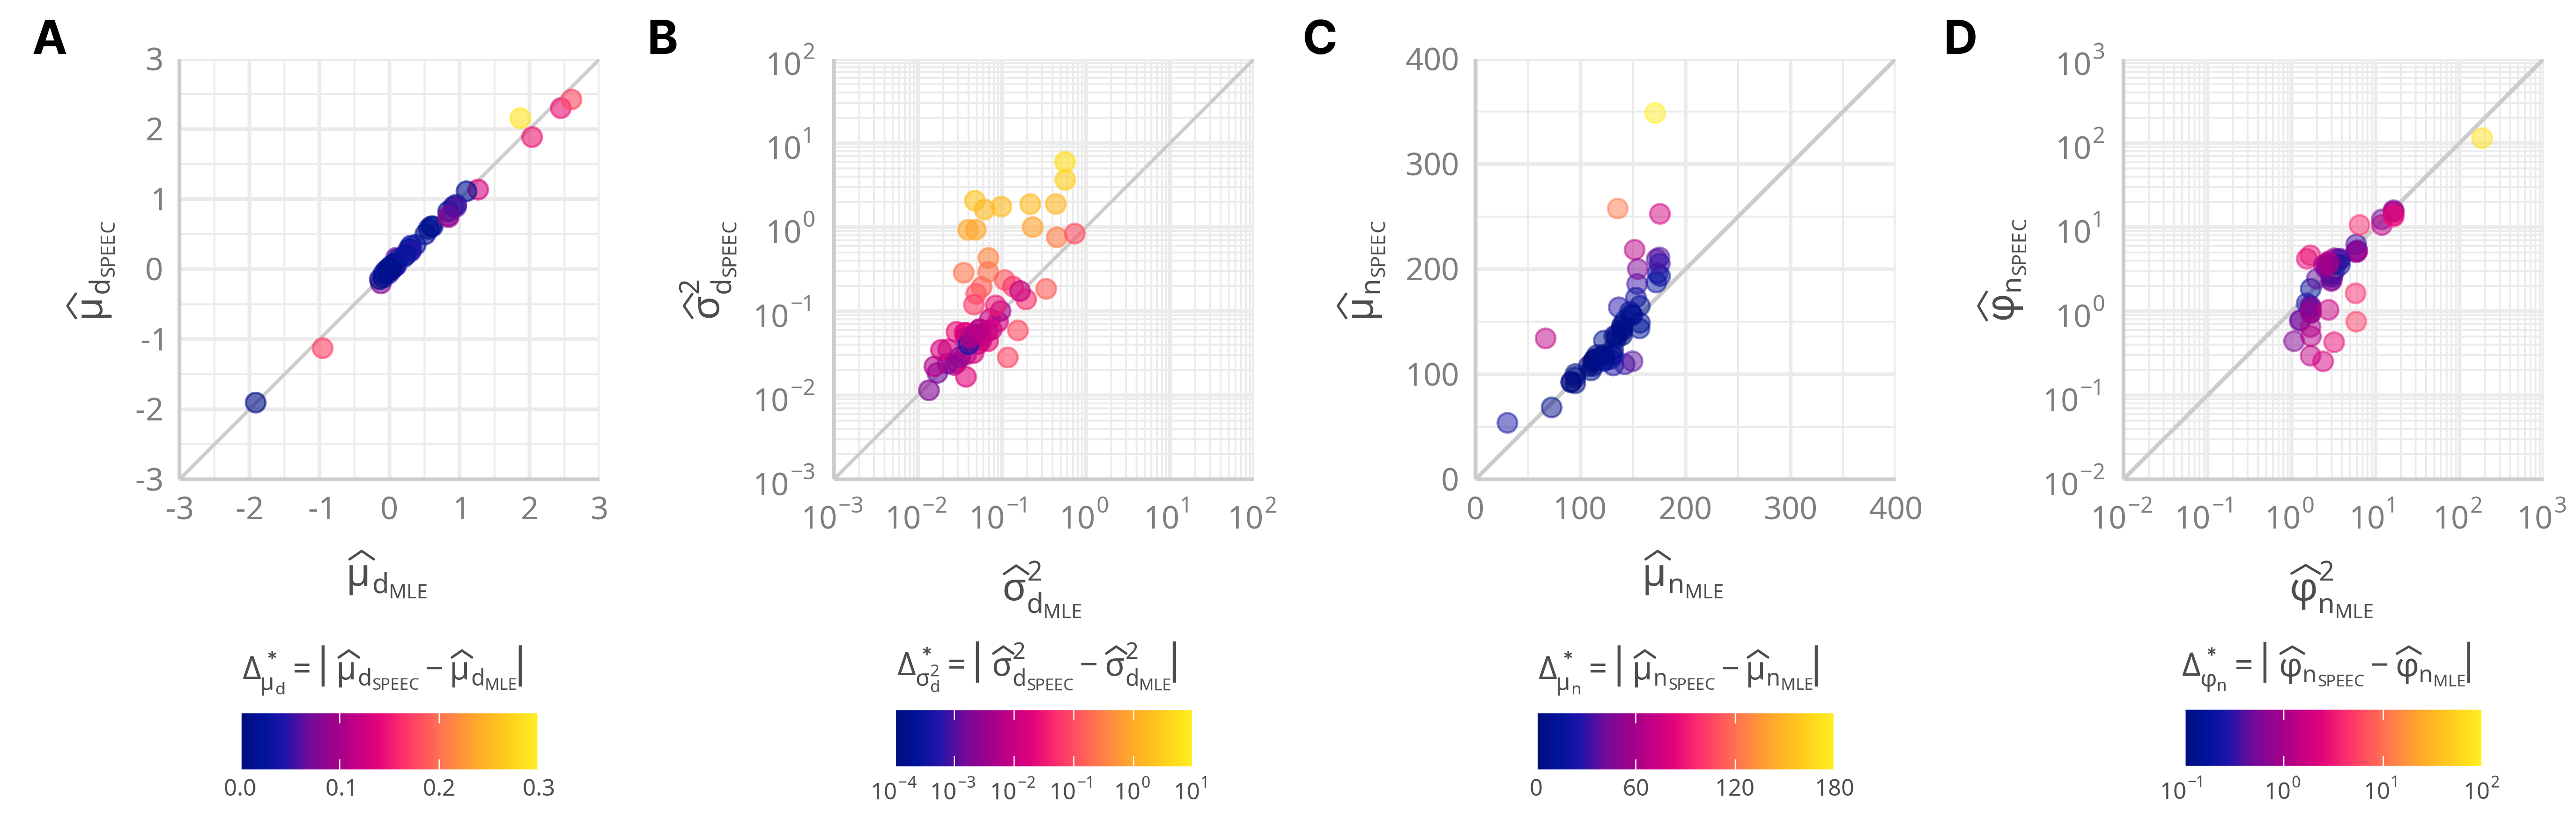
\includegraphics[width=1\textwidth,height=\textheight]{../figures/method_comparison.png}
\end{center}

\begingroup
\scriptsize
\textit{Note.} \textbf{A1}. Comparison of estimated mean parameter $\mu_d$ from Gaussian effect size distribution. \textbf{A2}. Comparison of estimated variance parameter $\sigma_d^2$ of Gaussian effect size distribution. Axes and colorbar are log (base 10) transformed. \textbf{B1}. Comparison of mean parameter $\mu_n$ of Negative-Binomial sample size distribution \textbf{B2}. Comparison of dispersion parameter $\phi_n$ of Negative-Binomial sample size distribution. Axes and colorbar are log (base 10) transformed.
\endgroup
\end{figure}

Regarding question one, Figure 3 provides a visual summary of the
analysis comparing the distributional parameters estimated by the SPEEC
method against those estimated by Maximum Likelihood Estimation (MLE).
The diagonal line signifies perfect alignment between MLE and SPEEC
estimates. Values below the diagonal indicate higher values for MLE
compared to SPEEC, while values above the diagonal indicate the
opposite.

Panel A of figure XX reiterates the findings of the analysis of
\(\mathcal{H}_3\), suggesting a small discrepancy between the two
methods in estimating the mean of the Gaussian effect size distribution,
\(M({\Delta_{\mu_d}})\) = -0.03, \(Mdn({\Delta_{\mu_d}})\) = -0.02. This
discrepancy can be deemed practically negligible according to the
equivalence test of \(\mathcal{H}_3\). However, the other panels
indicate contrasting outcomes.Panel B reveils a systematic discepancy in
the estimation of the variance parameter of the Gaussien effect size
distribution between SPEEC and MLE, \(M({\Delta_{\sigma^2_d}})\) = 0.59,
\(Mdn({\Delta_{\sigma^2_d}})\) = 0.11. Descriptively, this suggests that
on average, the variance was estimated to be greater in the SPEEC
approach compared to MLE. Furthermore, this discrepancy increases in
exponential trend and displays substantial heteroscedasticity with
rising variance estimates from the MLE approach. Similarly, Panel C also
illustrates a systematic overestimation of the mean parameter of the
Negative-Binomial sample size distribution by SPEEC in comparison to MLE
(\(M({\Delta_{\mu_n}})\) = 46.96, \(Mdn({\Delta_{\mu_n}})\) = 3.52),
which again increases in an exponential trend with higher mean parameter
estimates from MLE. Lastly, Panel D shows that the SPEEC approach
generally understimates dispersion parameter of the sample size
distribution in comparison to the ML estimate (\(M({\Delta_{\phi_n}})\)
= -2.02, \(Mdn({\Delta_{\phi_n}})\) = -0.19) and also furthermore
indicates a systematic relationship in the discrepancy between the two
approaches.

\begin{table}[H]
\centering\centering
\caption{Pairwise Pearson Correlations between the Absolute Difference of the Distributional Parameters from SPEEC and ML, Publication Bias Parameter and Meta-Analysis Size}
\centering
\resizebox{\ifdim\width>\linewidth\linewidth\else\width\fi}{!}{
\begin{threeparttable}
\fontsize{10}{12}\selectfont
\begin{tabular}[t]{>{\raggedright\arraybackslash}p{1.3cm}>{\centering\arraybackslash}p{3.5cm}>{\centering\arraybackslash}p{3.5cm}>{\centering\arraybackslash}p{2.75cm}>{\centering\arraybackslash}p{2.75cm}>{\centering\arraybackslash}p{2.2cm}}
\toprule
Variable & $\omega_{\text{PBS}}$ & $\lvert\Delta_{\mu_d}\rvert$ & $\lvert\Delta_{\sigma^2_d}\rvert$ & $\lvert\Delta_{\phi_n}\rvert$ & $\lvert\Delta_{\mu_n}\rvert$\\
\midrule
$\omega_{\text{PBS}}$ &  &  &  &  & \\
$\lvert\Delta_{\mu_d}\rvert$ & -0.44*** [-0.61, -0.23] &  &  &  & \\
$\lvert\Delta_{\sigma^2_d}\rvert$ & -0.37** [-0.56, -0.14] & 0.67*** [0.54, 0.76] &  &  & \\
$\lvert\Delta_{\phi_n}\rvert$ & 0.08 [-0.18, 0.33] & -0.06 [-0.31, 0.2] & -0.05 [-0.3, 0.21] &  & \\
$\lvert\Delta_{\mu_n}\rvert$ & 0.03 [-0.23, 0.29] & 0.15 [-0.11, 0.39] & 0.04 [-0.22, 0.3] & -0.05 [-0.3, 0.21] & \\
\addlinespace
$k$ & -0.14 [-0.38, 0.12] & 0.04 [-0.22, 0.29] & 0.15 [-0.11, 0.39] & -0.17 [-0.41, 0.09] & 0 [-0.26, 0.26]\\
\bottomrule
\end{tabular}
\begin{tablenotes}
\item \textit{Note.} Computed $p$-values are corrected for multiple comparison using the correction by Benjamini \& Hochberg (1995). $\lvert\Delta\rvert$ is the absolute difference for each distributional parameter between SPEEC and MLE.
\item[*] Significance *** $p$ < .001; ** $p$ < .01; * $p$ < .05
\end{tablenotes}
\end{threeparttable}}
\end{table}

To address the remaining diagnostic questions, we conducted a pairwise
correlational analysis between the absolute differences of the parameter
estimates derived from the two estimation methods, alongside the
publication bias parameter \(\widehat{\omega}_{\text{PBS}}\) and the
total number of primary replication studies \(k\) within each multisite
replication project or registered report. We used the Pearson
correlation coefficient and corrected the obtained \emph{p}-values for
multiple comparisons to control the false discovery rate
(\citeproc{ref-benjamini_controlling_1995}{Benjamini \& Hochberg,
1995}).

Regarding the parameters of the Gaussian effect size distribution, a
strong positive correlation was observed between the absolute difference
in the mean parameter estimates and the variance parameter estimates
obtained from ML and SPEEC. This indicates that as the absolute
discrepancy between SPEEC and ML increased for the mean parameter
\(\mu_d\), the absolute discrepancy also increased for the variance
parameter \(\sigma^2_d\) of the effect size distribution. Furthermore,
strong negative correlations were found between the publication bias
parameter \(\pbs\) and the discrepancy between ML and SPEEC estimates of
the mean and variance parameters of the effect size distribution. More
specifically, as the absolute discrepancy between both estimation
methods increased for both the mean (\(\lvert\Delta_{\mu_d}\rvert\)) and
variance (\(\lvert\Delta_{\sigma^2_d}\rvert\)), the publication bias
parameter \(\pbs\) decreased, signifying more severe predicted
publication bias. Notably, the total number of of primary replications
\(k\) was not significantly associated to the divergence of ML and SPEEC
of any distributional parameter or the publication bias parameter
\(\pbs\).

\newpage

\section{Discussion}\label{discussion}

\begin{itemize}
\tightlist
\item
  Analysis four theoretical predictions that should hold true, if the
  approach works in principle -\textgreater{} or phrased oppositely, if
  we don´t find evidence for the hypotheses -\textgreater{} there are
  problems
\end{itemize}

\emph{Confirmatory findings:}:

\begin{itemize}
\tightlist
\item
  Out of the four hypotheses, we found evidence for three predictions
  (speaking statistically) -\textgreater{} H1, H2, H3
\item
  No evidence that publication bias parameter is greater (less severe
  publication bias) in registered replication reports in comparison to
  traditional meta-analyses -\textgreater{} concerning result
  -\textgreater{} motivated the additional exploratory diagnostic
  analyses to assess potential problems of the parameter optimization
\end{itemize}

\emph{Exploratory findings:}:

\textbf{Q1:}

\begin{itemize}
\tightlist
\item
  There are differences between the the ML and SPEEC estimates
  -\textgreater{} for variance of effect size distribution, and mean and
  dispersion parameter of sample size distribution
\item
  These differences are not unsystematic across the entire range of the
  distributional parameters estimated via ML but rather show systematic
  trends (e.g.,)
\end{itemize}

\begin{itemize}
\tightlist
\item
  Proof of concept study -\textgreater{} not an comprehensive
  assessement of SPEEC appraoch
\end{itemize}

\begin{itemize}
\tightlist
\item
  Possibility of including:

  \begin{itemize}
  \tightlist
  \item
    Heterogeneity parameter \(\tau^2\) -\textgreater{} this could be
    very valuable
  \item
    Different effect size and thus different marginal distributions
    (thats the flexible aspect of SPEEC) -\textgreater{} odds ratio (log
    odds ratio), R2 variance
  \item
    Sample size planning parameter -\textgreater{} publiction bias not
    the only thing affecting n-es distribution
  \end{itemize}

  ```
\end{itemize}

\begin{itemize}
\tightlist
\item
  We did not find working approach for parameter optimization of the
  study -\textgreater{} this should/could be the focus of future studies
\item
  Framework has several areas which could be responsible for
  optimization problems

  \begin{itemize}
  \tightlist
  \item
    The choice of grid size
  \end{itemize}
\item
  Need for larger simulations study

  \begin{itemize}
  \tightlist
  \item
    Systematically vary: heterogeneity, true effect size, publication
    bias severity, meta-analysis study size \(k\)
  \item
    But also the control parameters of the SPEEC approach could be
    varied to see if systematic misestimation lies within here
  \item
    For example: grid size choice for KDE has direct influece on the the
    loss function (KL-divergence) for the optimization -\textgreater{}
    fine grid size for low sample size studies could be problematic
    (because of too much uncertainty), while very coarse grid size could
    be also problematic (because then differences between regarding
    publication bias parameter cannot be captured anymore)
  \end{itemize}
\item
  Flexibility of SPEEC approach (extending SPEEC):

  \begin{itemize}
  \tightlist
  \item
    Possibility to include heterogeneity parameter (deviations from the
    true effect size not only due to sampling error but)
  \item
    Possibility to include other influences on the sample size
    distribution -\textgreater{} sample size planning
  \item
    Possibility to use other marginal distribution for sample size
    distribution (depending on the data)
  \end{itemize}
\end{itemize}

\newpage

\section{References}\label{references}

\phantomsection\label{refs}
\begin{CSLReferences}{1}{0}
\bibitem[\citeproctext]{ref-allaire_quarto_2024}
Allaire, J. J., Teague, C., Scheidegger, C., Xie, Y., \& Dervieux, C.
(2024). \emph{Quarto}. \url{https://doi.org/10.5281/zenodo.5960048}

\bibitem[\citeproctext]{ref-andrade_p_2019}
Andrade, C. (2019). The {P} {Value} and {Statistical} {Significance}:
{Misunderstandings}, {Explanations}, {Challenges}, and {Alternatives}.
\emph{Indian Journal of Psychological Medicine}, \emph{41}(3), 210--215.
\url{https://doi.org/10.4103/IJPSYM.IJPSYM_193_19}

\bibitem[\citeproctext]{ref-arel-bundock_marginaleffects_2024}
Arel-Bundock, V. (2024). \emph{Marginaleffects: {Predictions},
{Comparisons}, {Slopes}, {Marginal} {Means}, and {Hypothesis} {Tests}}.
\url{https://marginaleffects.com/}

\bibitem[\citeproctext]{ref-bakan_test_1966}
Bakan, D. (1966). The test of significance in psychological research.
\emph{Psychological Bulletin}, \emph{66}(6), 423--437.
\url{https://doi.org/10.1037/h0020412}

\bibitem[\citeproctext]{ref-begg_publication_1994}
Begg, C. B. (1994). Publication bias. In \emph{The handbook of research
synthesis} (pp. 399--409). Russell Sage Foundation.

\bibitem[\citeproctext]{ref-begg_operating_1994}
Begg, C. B., \& Mazumdar, M. (1994). Operating {Characteristics} of a
{Rank} {Correlation} {Test} for {Publication} {Bias}. \emph{Biometrics},
\emph{50}(4), 1088--1101. \url{https://doi.org/10.2307/2533446}

\bibitem[\citeproctext]{ref-benjamini_controlling_1995}
Benjamini, Y., \& Hochberg, Y. (1995). Controlling the {False}
{Discovery} {Rate}: {A} {Practical} and {Powerful} {Approach} to
{Multiple} {Testing}. \emph{Journal of the Royal Statistical Society.
Series B (Methodological)}, \emph{57}(1), 289--300.
\url{https://www.jstor.org/stable/2346101}

\bibitem[\citeproctext]{ref-bozarth_signifying_1972}
Bozarth, J. D., \& Roberts, R. R. (1972). Signifying significant
significance. \emph{American Psychologist}, \emph{27}(8), 774--775.
\url{https://doi.org/10.1037/h0038034}

\bibitem[\citeproctext]{ref-cafri_meta-meta-analysis_2010}
Cafri, G., Kromrey, J. D., \& Brannick, M. T. (2010). A
{Meta}-{Meta}-{Analysis}: {Empirical} {Review} of {Statistical} {Power},
{Type} {I} {Error} {Rates}, {Effect} {Sizes}, and {Model} {Selection} of
{Meta}-{Analyses} {Published} in {Psychology}. \emph{Multivariate
Behavioral Research}, \emph{45}(2), 239--270.
\url{https://doi.org/10.1080/00273171003680187}

\bibitem[\citeproctext]{ref-camerer_evaluating_2018}
Camerer, C. F., Dreber, A., Holzmeister, F., Ho, T.-H., Huber, J.,
Johannesson, M., Kirchler, M., Nave, G., Nosek, B. A., Pfeiffer, T.,
Altmejd, A., Buttrick, N., Chan, T., Chen, Y., Forsell, E., Gampa, A.,
Heikensten, E., Hummer, L., Imai, T., \ldots{} Wu, H. (2018). Evaluating
the replicability of social science experiments in {Nature} and
{Science} between 2010 and 2015. \emph{Nature Human Behaviour},
\emph{2}(9), 637--644. \url{https://doi.org/10.1038/s41562-018-0399-z}

\bibitem[\citeproctext]{ref-chambers_past_2022}
Chambers, C. D., \& Tzavella, L. (2022). The past, present and future of
{Registered} {Reports}. \emph{Nature Human Behaviour}, \emph{6}(1),
29--42. \url{https://doi.org/10.1038/s41562-021-01193-7}

\bibitem[\citeproctext]{ref-cohen_earth_1994}
Cohen, J. (1994). The earth is round (p {\textless{}} .05).
\emph{American Psychologist}, \emph{49}(12), 997--1003.
\url{https://doi.org/10.1037/0003-066X.49.12.997}

\bibitem[\citeproctext]{ref-cooper_research_2019}
Cooper, H., Hedges, L. V., \& Valentine, J. C. (2019). Research
synthesis as a scientific process. In H. Cooper, L. V. Hedges, \& J. C.
Valentine (Eds.), \emph{The handbook of research synthesis and
meta-analysis} (3rd ed., pp. 3--16). Russell Sage Foundation.
\url{http://www.scopus.com/inward/record.url?scp=84902712953&partnerID=8YFLogxK}

\bibitem[\citeproctext]{ref-cribari-neto_beta_2010}
Cribari-Neto, F., \& Zeileis, A. (2010). Beta {Regression} in {R}.
\emph{Journal of Statistical Software}, \emph{34}, 1--24.
\url{https://doi.org/10.18637/jss.v034.i02}

\bibitem[\citeproctext]{ref-delacre_why_2017}
Delacre, M., Lakens, D., \& Leys, C. (2017). Why psychologists should by
default use {Welch}'s t-test instead of student's t-test.
\emph{International Review of Social Psychology}, \emph{30}(1), 92--101.
\url{https://doi.org/10.5334/irsp.82}

\bibitem[\citeproctext]{ref-dickersin_existence_1990}
Dickersin, K. (1990).
\href{https://www.ncbi.nlm.nih.gov/pubmed/2406472}{The existence of
publication bias and risk factors for its occurrence}. \emph{JAMA},
\emph{263}(10), 1385--1389.

\bibitem[\citeproctext]{ref-dickersin_publication_1993}
Dickersin, K., \& Min, Y.-I. (1993). Publication {Bias}: {The} {Problem}
{That} {Won}'t {Go} {Away}. \emph{Annals of the New York Academy of
Sciences}, \emph{703}(1), 135--148.
\url{https://doi.org/10.1111/j.1749-6632.1993.tb26343.x}

\bibitem[\citeproctext]{ref-ebersole_many_2016}
Ebersole, C. R., Atherton, O. E., Belanger, A. L., Skulborstad, H. M.,
Allen, J. M., Banks, J. B., Baranski, E., Bernstein, M. J., Bonfiglio,
D. B. V., Boucher, L., Brown, E. R., Budiman, N. I., Cairo, A. H.,
Capaldi, C. A., Chartier, C. R., Chung, J. M., Cicero, D. C., Coleman,
J. A., Conway, J. G., \ldots{} Nosek, B. A. (2016). Many {Labs} 3:
{Evaluating} participant pool quality across the academic semester via
replication. \emph{Journal of Experimental Social Psychology},
\emph{67}, 68--82. \url{https://doi.org/10.1016/j.jesp.2015.10.012}

\bibitem[\citeproctext]{ref-ebersole_many_2020}
Ebersole, C. R., Mathur, M. B., Baranski, E., Bart-Plange, D.-J.,
Buttrick, N. R., Chartier, C. R., Corker, K. S., Corley, M., Hartshorne,
J. K., IJzerman, H., Lazarević, L. B., Rabagliati, H., Ropovik, I.,
Aczel, B., Aeschbach, L. F., Andrighetto, L., Arnal, J. D., Arrow, H.,
Babincak, P., \ldots{} Nosek, B. A. (2020). Many {Labs} 5: {Testing}
{Pre}-{Data}-{Collection} {Peer} {Review} as an {Intervention} to
{Increase} {Replicability}. \emph{Advances in Methods and Practices in
Psychological Science}, \emph{3}(3), 309--331.
\url{https://doi.org/10.1177/2515245920958687}

\bibitem[\citeproctext]{ref-edelbuettel_rcppde_2022}
Edelbuettel, D. (2022). \emph{{RcppDE}: {Global} {Optimization} by
{Differential} {Evolution} in {C}++}.
\url{https://cran.r-project.org/web/packages/RcppDE/index.html}

\bibitem[\citeproctext]{ref-egger_bias_1997}
Egger, M., Davey Smith, G., Schneider, M., \& Minder, C. (1997). Bias in
meta-analysis detected by a simple, graphical test. \emph{BMJ (Clinical
Research Ed.)}, \emph{315}(7109), 629--634.
\url{https://doi.org/10.1136/bmj.315.7109.629}

\bibitem[\citeproctext]{ref-feoktistov_differential_2006}
Feoktistov, V. (2006). \emph{Differential {Evolution} -- {In} {Search}
of {Solutions}} (Vol. 5). Springer.
\url{https://doi.org/10.1007/978-0-387-36896-2}

\bibitem[\citeproctext]{ref-ferrari_beta_2004}
Ferrari, S., \& Cribari-Neto, F. (2004). Beta {Regression} for
{Modelling} {Rates} and {Proportions}. \emph{Journal of Applied
Statistics}, \emph{31}(7), 799--815.
\url{https://doi.org/10.1080/0266476042000214501}

\bibitem[\citeproctext]{ref-franco_publication_2014}
Franco, A., Malhotra, N., \& Simonovits, G. (2014). Publication bias in
the social sciences: {Unlocking} the file drawer. \emph{Science},
\emph{345}(6203), 1502--1505.
\url{https://doi.org/10.1126/science.1255484}

\bibitem[\citeproctext]{ref-fritz_comprehensive_2013}
Fritz, A., Scherndl, T., \& Kühberger, A. (2013). A comprehensive review
of reporting practices in psychological journals: {Are} effect sizes
really enough? \emph{Theory \& Psychology}, \emph{23}(1), 98--122.
\url{https://doi.org/10.1177/0959354312436870}

\bibitem[\citeproctext]{ref-gerber_testing_2001}
Gerber, A. S., Green, D. P., \& Nickerson, D. (2001). Testing for
{Publication} {Bias} in {Political} {Science}. \emph{Political
Analysis}, \emph{9}(4), 385--392.
\url{https://www.jstor.org/stable/25791658}

\bibitem[\citeproctext]{ref-ghoreishi_termination_2017}
Ghoreishi, N., Clausen, A., \& Jørgensen, B. N. (2017). Termination
{Criteria} in {Evolutionary} {Algorithms}: {A} {Survey}.
\emph{Proceedings of 9th {International} {Joint} {Conference} on
{Computational} {Intelligence}}, \emph{1}, 373--384.
\url{https://doi.org/10.5220/0006577903730384}

\bibitem[\citeproctext]{ref-harrer_doing_2021}
Harrer, M., Cuijpers, P., A, F. T., \& Ebert, D. D. (2021). \emph{Doing
{Meta}-{Analysis} {With} {R}: {A} {Hands}-{On} {Guide}} (1st ed.).
Chapman \& Hall/CRC Press.

\bibitem[\citeproctext]{ref-hedges_modeling_1992}
Hedges, L. V. (1992). Modeling {Publication} {Selection} {Effects} in
{Meta}-{Analysis}. \emph{Statistical Science}, \emph{7}(2), 246--255.
\url{https://doi.org/10.1214/ss/1177011364}

\bibitem[\citeproctext]{ref-iyengar_selection_1988}
Iyengar, S., \& Greenhouse, J. B. (1988). Selection {Models} and the
{File} {Drawer} {Problem}. \emph{Statistical Science}, \emph{3}(1),
109--117. \url{https://www.jstor.org/stable/2245925}

\bibitem[\citeproctext]{ref-jain_termination_2001}
Jain, B. J., Pohlheim, H., \& Wegener, J. (2001). On termination
criteria of evolutionary algorithms. \emph{Proceedings of the 3rd
{Annual} {Conference} on {Genetic} and {Evolutionary} {Computation}},
768--768.

\bibitem[\citeproctext]{ref-jennions_publication_2002}
Jennions, M. D., \& Møller, A. P. (2002a). Publication bias in ecology
and evolution: An empirical assessment using the {``trim and fill''}
method. \emph{Biological Reviews}, \emph{77}(2), 211--222.
\url{https://doi.org/10.1017/S1464793101005875}

\bibitem[\citeproctext]{ref-jennions_relationships_2002}
Jennions, M. D., \& Møller, A. P. (2002b). Relationships fade with time:
A meta-analysis of temporal trends in publication in ecology and
evolution. \emph{Proceedings of the Royal Society B: Biological
Sciences}, \emph{269}(1486), 43--48.
\url{https://doi.org/10.1098/rspb.2001.1832}

\bibitem[\citeproctext]{ref-kicinski_how_2014}
Kicinski, M. (2014). How does under-reporting of negative and
inconclusive results affect the false-positive rate in meta-analysis?
{A} simulation study. \emph{BMJ Open}, \emph{4}(8), e004831.
\url{https://doi.org/10.1136/bmjopen-2014-004831}

\bibitem[\citeproctext]{ref-kitcher_advancement_1993}
Kitcher, P. (1993). \emph{The {Advancement} of {Science}: {Science}
{Without} {Legend}, {Objectivity} {Without} {Illusions}}. Oxford
University Press.

\bibitem[\citeproctext]{ref-klein_investigating_2014}
Klein, R. A., Ratliff, K. A., Vianello, M., Adams, R. B., Bahník, Š.,
Bernstein, M. J., Bocian, K., Brandt, M. J., Brooks, B., Brumbaugh, C.
C., Cemalcilar, Z., Chandler, J., Cheong, W., Davis, W. E., Devos, T.,
Eisner, M., Frankowska, N., Furrow, D., Galliani, E. M., \ldots{} Nosek,
B. A. (2014). Investigating variation in replicability: {A} "many labs"
replication project. \emph{Social Psychology}, \emph{45}(3), 142--152.
\url{https://doi.org/10.1027/1864-9335/a000178}

\bibitem[\citeproctext]{ref-klein_many_2018}
Klein, R. A., Vianello, M., Hasselman, F., Adams, B. G., Adams, R. B.,
Alper, S., Aveyard, M., Axt, J. R., Babalola, M. T., Bahník, Š., Batra,
R., Berkics, M., Bernstein, M. J., Berry, D. R., Bialobrzeska, O.,
Binan, E. D., Bocian, K., Brandt, M. J., Busching, R., \ldots{} Nosek,
B. A. (2018). Many {Labs} 2: {Investigating} {Variation} in
{Replicability} {Across} {Samples} and {Settings}. \emph{Advances in
Methods and Practices in Psychological Science}, \emph{1}(4), 443--490.
\url{https://doi.org/10.1177/2515245918810225}

\bibitem[\citeproctext]{ref-kuhberger_publication_2014}
Kühberger, A., Fritz, A., \& Scherndl, T. (2014). Publication {Bias} in
{Psychology}: {A} {Diagnosis} {Based} on the {Correlation} between
{Effect} {Size} and {Sample} {Size}. \emph{PLoS ONE}, \emph{9}(9),
e105825. \url{https://doi.org/10.1371/journal.pone.0105825}

\bibitem[\citeproctext]{ref-kullback_information_1951}
Kullback, S., \& Leibler, R. A. (1951). On {Information} and
{Sufficiency}. \emph{The Annals of Mathematical Statistics},
\emph{22}(1), 79--86. \url{https://doi.org/10.1214/aoms/1177729694}

\bibitem[\citeproctext]{ref-lakens_performing_2014}
Lakens, D. (2014). Performing high-powered studies efficiently with
sequential analyses. \emph{European Journal of Social Psychology},
\emph{44}(7), 701--710. \url{https://doi.org/10.1002/ejsp.2023}

\bibitem[\citeproctext]{ref-lakens_equivalence_2017}
Lakens, D. (2017). Equivalence {Tests}: {A} {Practical} {Primer} for t
{Tests}, {Correlations}, and {Meta}-{Analyses}. \emph{Social
Psychological and Personality Science}, \emph{8}(4), 355--362.
\url{https://doi.org/10.1177/1948550617697177}

\bibitem[\citeproctext]{ref-lakens_toster_2023}
Lakens, D., \& Caldwell, A. (2023). \emph{{TOSTER}: {Two} {One}-{Sided}
{Tests} ({TOST}) {Equivalence} {Testing}}.
\url{https://cran.r-project.org/web/packages/TOSTER/index.html}

\bibitem[\citeproctext]{ref-lakens_improving_2020}
Lakens, D., McLatchie, N., Isager, P. M., Scheel, A. M., \& Dienes, Z.
(2020). Improving {Inferences} {About} {Null} {Effects} {With} {Bayes}
{Factors} and {Equivalence} {Tests}. \emph{The Journals of Gerontology:
Series B}, \emph{75}(1), 45--57.
\url{https://doi.org/10.1093/geronb/gby065}

\bibitem[\citeproctext]{ref-lakens_equivalence_2018}
Lakens, D., Scheel, A. M., \& Isager, P. M. (2018). Equivalence
{Testing} for {Psychological} {Research}: {A} {Tutorial}. \emph{Advances
in Methods and Practices in Psychological Science}, \emph{1}(2),
259--269. \url{https://doi.org/10.1177/2515245918770963}

\bibitem[\citeproctext]{ref-levine_sample_2009}
Levine, T. R., Asada, K. J., \& Carpenter, C. (2009). Sample {Sizes} and
{Effect} {Sizes} are {Negatively} {Correlated} in {Meta}-{Analyses}:
{Evidence} and {Implications} of a {Publication} {Bias} {Against}
{NonSignificant} {Findings}. \emph{Communication Monographs},
\emph{76}(3), 286--302. \url{https://doi.org/10.1080/03637750903074685}

\bibitem[\citeproctext]{ref-light_summing_1984}
Light, R., \& Pillemer, D. (1984). \emph{Summing up: {The} science of
reviewing research.} Harvard University Press.
\url{https://scholars.unh.edu/psych_facpub/194}

\bibitem[\citeproctext]{ref-linden_heterogeneity_2021}
Linden, A. H., \& Hönekopp, J. (2021). Heterogeneity of {Research}
{Results}: {A} {New} {Perspective} {From} {Which} to {Assess} and
{Promote} {Progress} in {Psychological} {Science}. \emph{Perspectives on
Psychological Science}, \emph{16}(2), 358--376.
\url{https://doi.org/10.1177/1745691620964193}

\bibitem[\citeproctext]{ref-linden_publication_2024}
Linden, A., Pollet, T. V., \& Hönekopp, J. (2024). \emph{Publication
{Bias} in {Psychology}: {A} {Closer} {Look} at the {Correlation}
{Between} {Sample} {Size} and {Effect} {Size}}.
\url{https://doi.org/10.31234/osf.io/s4znd}

\bibitem[\citeproctext]{ref-lovakov_empirically_2021}
Lovakov, A., \& Agadullina, E. R. (2021). Empirically derived guidelines
for effect size interpretation in social psychology. \emph{European
Journal of Social Psychology}, \emph{51}(3), 485--504.
\url{https://doi.org/10.1002/ejsp.2752}

\bibitem[\citeproctext]{ref-marks-anglin_historical_2020}
Marks-Anglin, A., \& Chen, Y. (2020). A historical review of publication
bias. \emph{Research Synthesis Methods}, \emph{11}(6), 725--742.
\url{https://doi.org/10.1002/jrsm.1452}

\bibitem[\citeproctext]{ref-marszalek_sample_2011}
Marszalek, J. M., Barber, C., Kohlhart, J., \& Holmes, C. B. (2011).
Sample size in psychological research over the past 30 years.
\emph{Perceptual and Motor Skills}, \emph{112}(2), 331--348.
\url{https://doi.org/10.2466/03.11.PMS.112.2.331-348}

\bibitem[\citeproctext]{ref-mcshane_abandon_2019}
McShane, B. B., Gal, D., Gelman, A., Robert, C., \& Tackett, J. L.
(2019). Abandon {Statistical} {Significance}. \emph{The American
Statistician}, \emph{73}(sup1), 235--245.
\url{https://doi.org/10.1080/00031305.2018.1527253}

\bibitem[\citeproctext]{ref-merkel_docker_2014}
Merkel, D. (2014). Docker: Lightweight {Linux} containers for consistent
development and deployment. \emph{Linux Journal}, \emph{2014}(239), 2:2.

\bibitem[\citeproctext]{ref-molder_sustainable_2021}
Mölder, F., Jablonski, K. P., Letcher, B., Hall, M. B., Tomkins-Tinch,
C. H., Sochat, V., Forster, J., Lee, S., Twardziok, S. O., Kanitz, A.,
Wilm, A., Holtgrewe, M., Rahmann, S., Nahnsen, S., \& Köster, J. (2021).
\emph{Sustainable data analysis with {Snakemake}}. F1000Research.
\url{https://doi.org/10.12688/f1000research.29032.1}

\bibitem[\citeproctext]{ref-moller_how_2001}
Møller, A., \& Jennions, M. (2001). How important are direct fitness
benefits of sexual selection? \emph{Naturwissenschaften}, \emph{88}(10),
401--415. \url{https://doi.org/10.1007/s001140100255}

\bibitem[\citeproctext]{ref-munafo_how_2010}
Munafò, M. R., \& Flint, J. (2010). How reliable are scientific studies?
\emph{The British Journal of Psychiatry}, \emph{197}(4), 257--258.
\url{https://doi.org/10.1192/bjp.bp.109.069849}

\bibitem[\citeproctext]{ref-munafo_manifesto_2017}
Munafò, M. R., Nosek, B. A., Bishop, D. V. M., Button, K. S., Chambers,
C. D., Percie du Sert, N., Simonsohn, U., Wagenmakers, E.-J., Ware, J.
J., \& Ioannidis, J. P. A. (2017). A manifesto for reproducible science.
\emph{Nature Human Behaviour}, \emph{1}(1), 1--10.
\url{https://doi.org/10.1038/s41562-016-0021}

\bibitem[\citeproctext]{ref-nelder_simplex_1965}
Nelder, J. A., \& Mead, R. (1965). A {Simplex} {Method} for {Function}
{Minimization}. \emph{The Computer Journal}, \emph{7}(4), 308--313.
\url{https://doi.org/10.1093/comjnl/7.4.308}

\bibitem[\citeproctext]{ref-nosek_registered_2014}
Nosek, B. A., \& Lakens, D. (2014). Registered {Reports}: {A} {Method}
to {Increase} the {Credibility} of {Published} {Results}. \emph{Social
Psychology}, \emph{45}(3), 137--141.
\url{https://doi.org/10.1027/1864-9335/a000192}

\bibitem[\citeproctext]{ref-nosek_scientific_2012}
Nosek, B. A., Spies, J. R., \& Motyl, M. (2012). Scientific {Utopia}:
{II}. {Restructuring} {Incentives} and {Practices} to {Promote} {Truth}
{Over} {Publishability}. \emph{Perspectives on Psychological Science},
\emph{7}(6), 615--631. \url{https://doi.org/10.1177/1745691612459058}

\bibitem[\citeproctext]{ref-open_science_collaboration_estimating_2015}
Open Science Collaboration. (2015). Estimating the reproducibility of
psychological science. \emph{Science}, \emph{349}(6251), aac4716.
\url{https://doi.org/10.1126/science.aac4716}

\bibitem[\citeproctext]{ref-palmer_detecting_1999}
Palmer, A. R. (1999). Detecting {Publication} {Bias} in {Meta}‐analyses:
{A} {Case} {Study} of {Fluctuating} {Asymmetry} and {Sexual}
{Selection}. \emph{The American Naturalist}, \emph{154}(2), 220--233.
\url{https://doi.org/10.1086/303223}

\bibitem[\citeproctext]{ref-renkewitz_how_2019}
Renkewitz, F., \& Keiner, M. (2019). How to {Detect} {Publication}
{Bias} in {Psychological} {Research}. \emph{Zeitschrift Für
Psychologie}, \emph{227}(4), 261--279.
\url{https://doi.org/10.1027/2151-2604/a000386}

\bibitem[\citeproctext]{ref-rosenthal_file_1979}
Rosenthal, R. (1979). The file drawer problem and tolerance for null
results. \emph{Psychological Bulletin}, \emph{86}(3), 638--641.
\url{https://doi.org/10.1037/0033-2909.86.3.638}

\bibitem[\citeproctext]{ref-sassenberg_research_2019}
Sassenberg, K., \& Ditrich, L. (2019). Research in {Social} {Psychology}
{Changed} {Between} 2011 and 2016: {Larger} {Sample} {Sizes}, {More}
{Self}-{Report} {Measures}, and {More} {Online} {Studies}.
\emph{Advances in Methods and Practices in Psychological Science},
\emph{2}(2), 107--114. \url{https://doi.org/10.1177/2515245919838781}

\bibitem[\citeproctext]{ref-schuirmann_comparison_1987}
Schuirmann, D. J. (1987). A comparison of the {Two} {One}-{Sided}
{Tests} {Procedure} and the {Power} {Approach} for assessing the
equivalence of average bioavailability. \emph{Journal of
Pharmacokinetics and Biopharmaceutics}, \emph{15}(6), 657--680.
\url{https://doi.org/10.1007/BF01068419}

\bibitem[\citeproctext]{ref-sheather_reliable_1991}
Sheather, S. J., \& Jones, M. C. (1991). A {Reliable} {Data}-{Based}
{Bandwidth} {Selection} {Method} for {Kernel} {Density} {Estimation}.
\emph{Journal of the Royal Statistical Society. Series B
(Methodological)}, \emph{53}(3), 683--690.
\url{https://www.jstor.org/stable/2345597}

\bibitem[\citeproctext]{ref-shen_samples_2011}
Shen, W., Kiger, T. B., Davies, S. E., Rasch, R. L., Simon, K. M., \&
Ones, D. S. (2011). Samples in applied psychology: {Over} a decade of
research in review. \emph{Journal of Applied Psychology}, \emph{96}(5),
1055--1064. \url{https://doi.org/10.1037/a0023322}

\bibitem[\citeproctext]{ref-simons_introduction_2014}
Simons, D. J., Holcombe, A. O., \& Spellman, B. A. (2014). An
{Introduction} to {Registered} {Replication} {Reports} at {Perspectives}
on {Psychological} {Science}. \emph{Perspectives on Psychological
Science}, \emph{9}(5), 552--555.
\url{https://www.jstor.org/stable/44290039}

\bibitem[\citeproctext]{ref-slavin_effective_2008}
Slavin, R. E., Cheung, A., Groff, C., \& Lake, C. (2008). Effective
reading programs for middle and high schools: {A} best-evidence
synthesis. \emph{Reading Research Quarterly}, \emph{43}(3), 290--322.
\url{https://doi.org/10.1598/RRQ.43.3.4}

\bibitem[\citeproctext]{ref-slavin_relationship_2009}
Slavin, R., \& Smith, D. (2009). The {Relationship} {Between} {Sample}
{Sizes} and {Effect} {Sizes} in {Systematic} {Reviews} in {Education}.
\emph{Educational Evaluation and Policy Analysis}, \emph{31}(4),
500--506. \url{https://doi.org/10.3102/0162373709352369}

\bibitem[\citeproctext]{ref-smart_importance_1964}
Smart, R. G. (1964). The importance of negative results in psychological
research. \emph{Canadian Psychologist / Psychologie Canadienne},
\emph{5a}(4), 225--232. \url{https://doi.org/10.1037/h0083036}

\bibitem[\citeproctext]{ref-smithson_better_2006}
Smithson, M., \& Verkuilen, J. (2006). A better lemon squeezer?
{Maximum}-likelihood regression with beta-distributed dependent
variables. \emph{Psychological Methods}, \emph{11}(1), 54--71.
\url{https://doi.org/10.1037/1082-989X.11.1.54}

\bibitem[\citeproctext]{ref-song_dissemination_2010}
Song, F., Parekh, S., Hooper, L., Loke, Y. K., Ryder, J., Sutton, A. J.,
Hing, C., Kwok, C. S., Pang, C., \& Harvey, I. (2010). Dissemination and
publication of research findings : An updated review of related biases.
\emph{Health Technology Assessment}, \emph{14}(8), 1--220.
\url{https://doi.org/10.3310/hta14080}

\bibitem[\citeproctext]{ref-stanley_detecting_2021}
Stanley, T. D., Doucouliagos, H., Ioannidis, J. P. A., \& Carter, E. C.
(2021). Detecting publication selection bias through excess statistical
significance. \emph{Research Synthesis Methods}, \emph{12}(6), 776--795.
\url{https://doi.org/10.1002/jrsm.1512}

\bibitem[\citeproctext]{ref-sterling_publication_1959}
Sterling, T. D. (1959). Publication {Decisions} and their {Possible}
{Effects} on {Inferences} {Drawn} from {Tests} of {Significance}---or
{Vice} {Versa}. \emph{Journal of the American Statistical Association},
\emph{54}(285), 30--34.
\url{https://doi.org/10.1080/01621459.1959.10501497}

\bibitem[\citeproctext]{ref-storn_differential_1997}
Storn, R., \& Price, K. (1997). Differential {Evolution} -- {A} {Simple}
and {Efficient} {Heuristic} for global {Optimization} over {Continuous}
{Spaces}. \emph{Journal of Global Optimization}, \emph{11}(4), 341--359.
\url{https://doi.org/10.1023/A:1008202821328}

\bibitem[\citeproctext]{ref-szucs_empirical_2017}
Szucs, D., \& Ioannidis, J. P. A. (2017). Empirical assessment of
published effect sizes and power in the recent cognitive neuroscience
and psychology literature. \emph{PLOS Biology}, \emph{15}(3), e2000797.
\url{https://doi.org/10.1371/journal.pbio.2000797}

\bibitem[\citeproctext]{ref-r_core_team_r_2023}
Team, R. C. (2023). \emph{R: {A} {Language} and {Environment} for
{Statistical} {Computing}}. R Foundation for Statistical Computing.
\url{https://www.R-project.org}

\bibitem[\citeproctext]{ref-ushey_renv_2024}
Ushey, K., \& Wickham, H. (2024). \emph{Renv: {Project} {Environments}}.
\url{https://cran.r-project.org/web/packages/renv/index.html}

\bibitem[\citeproctext]{ref-vevea_publication_2019}
Vevea, J. L., Coburn, K., \& Sutton, A. J. (2019). Publication {Bias}.
In H. Cooper, L. V. Hedges, \& J. C. Valentine (Eds.), \emph{The
handbook of research synthesis and meta-analysis} (3rd ed., pp.
383--433). Russell Sage Foundation.

\bibitem[\citeproctext]{ref-weinerova_published_2022}
Weinerová, J., Szűcs, D., \& Ioannidis, J. P. A. (2022). Published
correlational effect sizes in social and developmental psychology.
\emph{Royal Society Open Science}, \emph{9}(12), 220311.
\url{https://doi.org/10.1098/rsos.220311}

\bibitem[\citeproctext]{ref-zeileis_betareg_2021}
Zeileis, A., Cribari-Neto, F., Gruen, B., Kosmidis, I., by), A. B. S.
(earlier. version, \& by), A. V. R. (earlier. version. (2021).
\emph{Betareg: {Beta} {Regression}}.
\url{https://cran.r-project.org/web/packages/betareg/index.html}

\end{CSLReferences}

\newpage
\renewcommand{\thetable}{\Alph{section}\arabic{table}}

\section{Appendix}\label{appendix}

\subsection{Appendix A: Power Analyses determining the
SESOIs}\label{appendix-a-power-analyses-determining-the-sesois}

The simulated-based sensitivity power analysis targeted a statistical
power of \(1-\beta=0.8\) with a fixed significance level of
\(\alpha = .05\). The simulated samples sizes were specified according
to the hypotheses as follows:

\begin{itemize}
\tightlist
\item
  \(\mathcal{H}_1\): \(n = 150\) (only traditional meta-analyses)
\item
  \(\mathcal{H}_2\) and \(\mathcal{H}_4\): \(n = 207\) (both traditional
  meta-analyses and multisite replication studies)
\item
  \(\mathcal{H}_3\): \(n = 57\) (only multisite replication studies)
\end{itemize}

The distributional assumptions for the four sensitivity power analyses
were specified as follows: \[
\mathcal{H}_1: \quad z_{r_S} \sim \mathcal{N}(\mu=-0.1, \sigma=0.5) \\
\]

\[
\mathcal{H}_2 ~ \text{and} ~ \mathcal{H}_3: \quad \Delta_{\mu_d} \sim \mathcal{N}\Big(\mu=0, \sigma_{diff}=\sqrt{0.3^2+0.3^2}\Big) 
\]

For hypothesis four, the proportions of the categorical predictor of the
research synthesis type (traditional meta-analysis \(MA\), multisite
replication \(MR\)) were chosen according the the actual proportions of
the data (\(n_{MA}=150, n_{MR}=57\)). For all simulations-based
sensitivity power analyses
(\(\mathcal{H}_1, \mathcal{H}_2, \mathcal{H}_4\)), the number of
simulations was set to \(n_{iter}=5000\). More over, the the
beta-regressions on \(\pbs\) in \(\mathcal{H}_1\), \(\mathcal{H}_2\),
and \(\mathcal{H}_4\) involved simulations for different dispersion
parameter conditions \(\phi = \{10, 20, 30\}\), as lower dispersion
parameters result in reduced test power. We set the SESOI for the
parameters of interest more conservatively, ensuring a minimum power of
80\% for the lowest dispersion parameter \(\phi = 10\).

\begin{figure}[H]
\caption{Power Curves of the Sensitivity Power Analyses determining the SESOIs
\label{fig:sesoi}}

\begin{center}
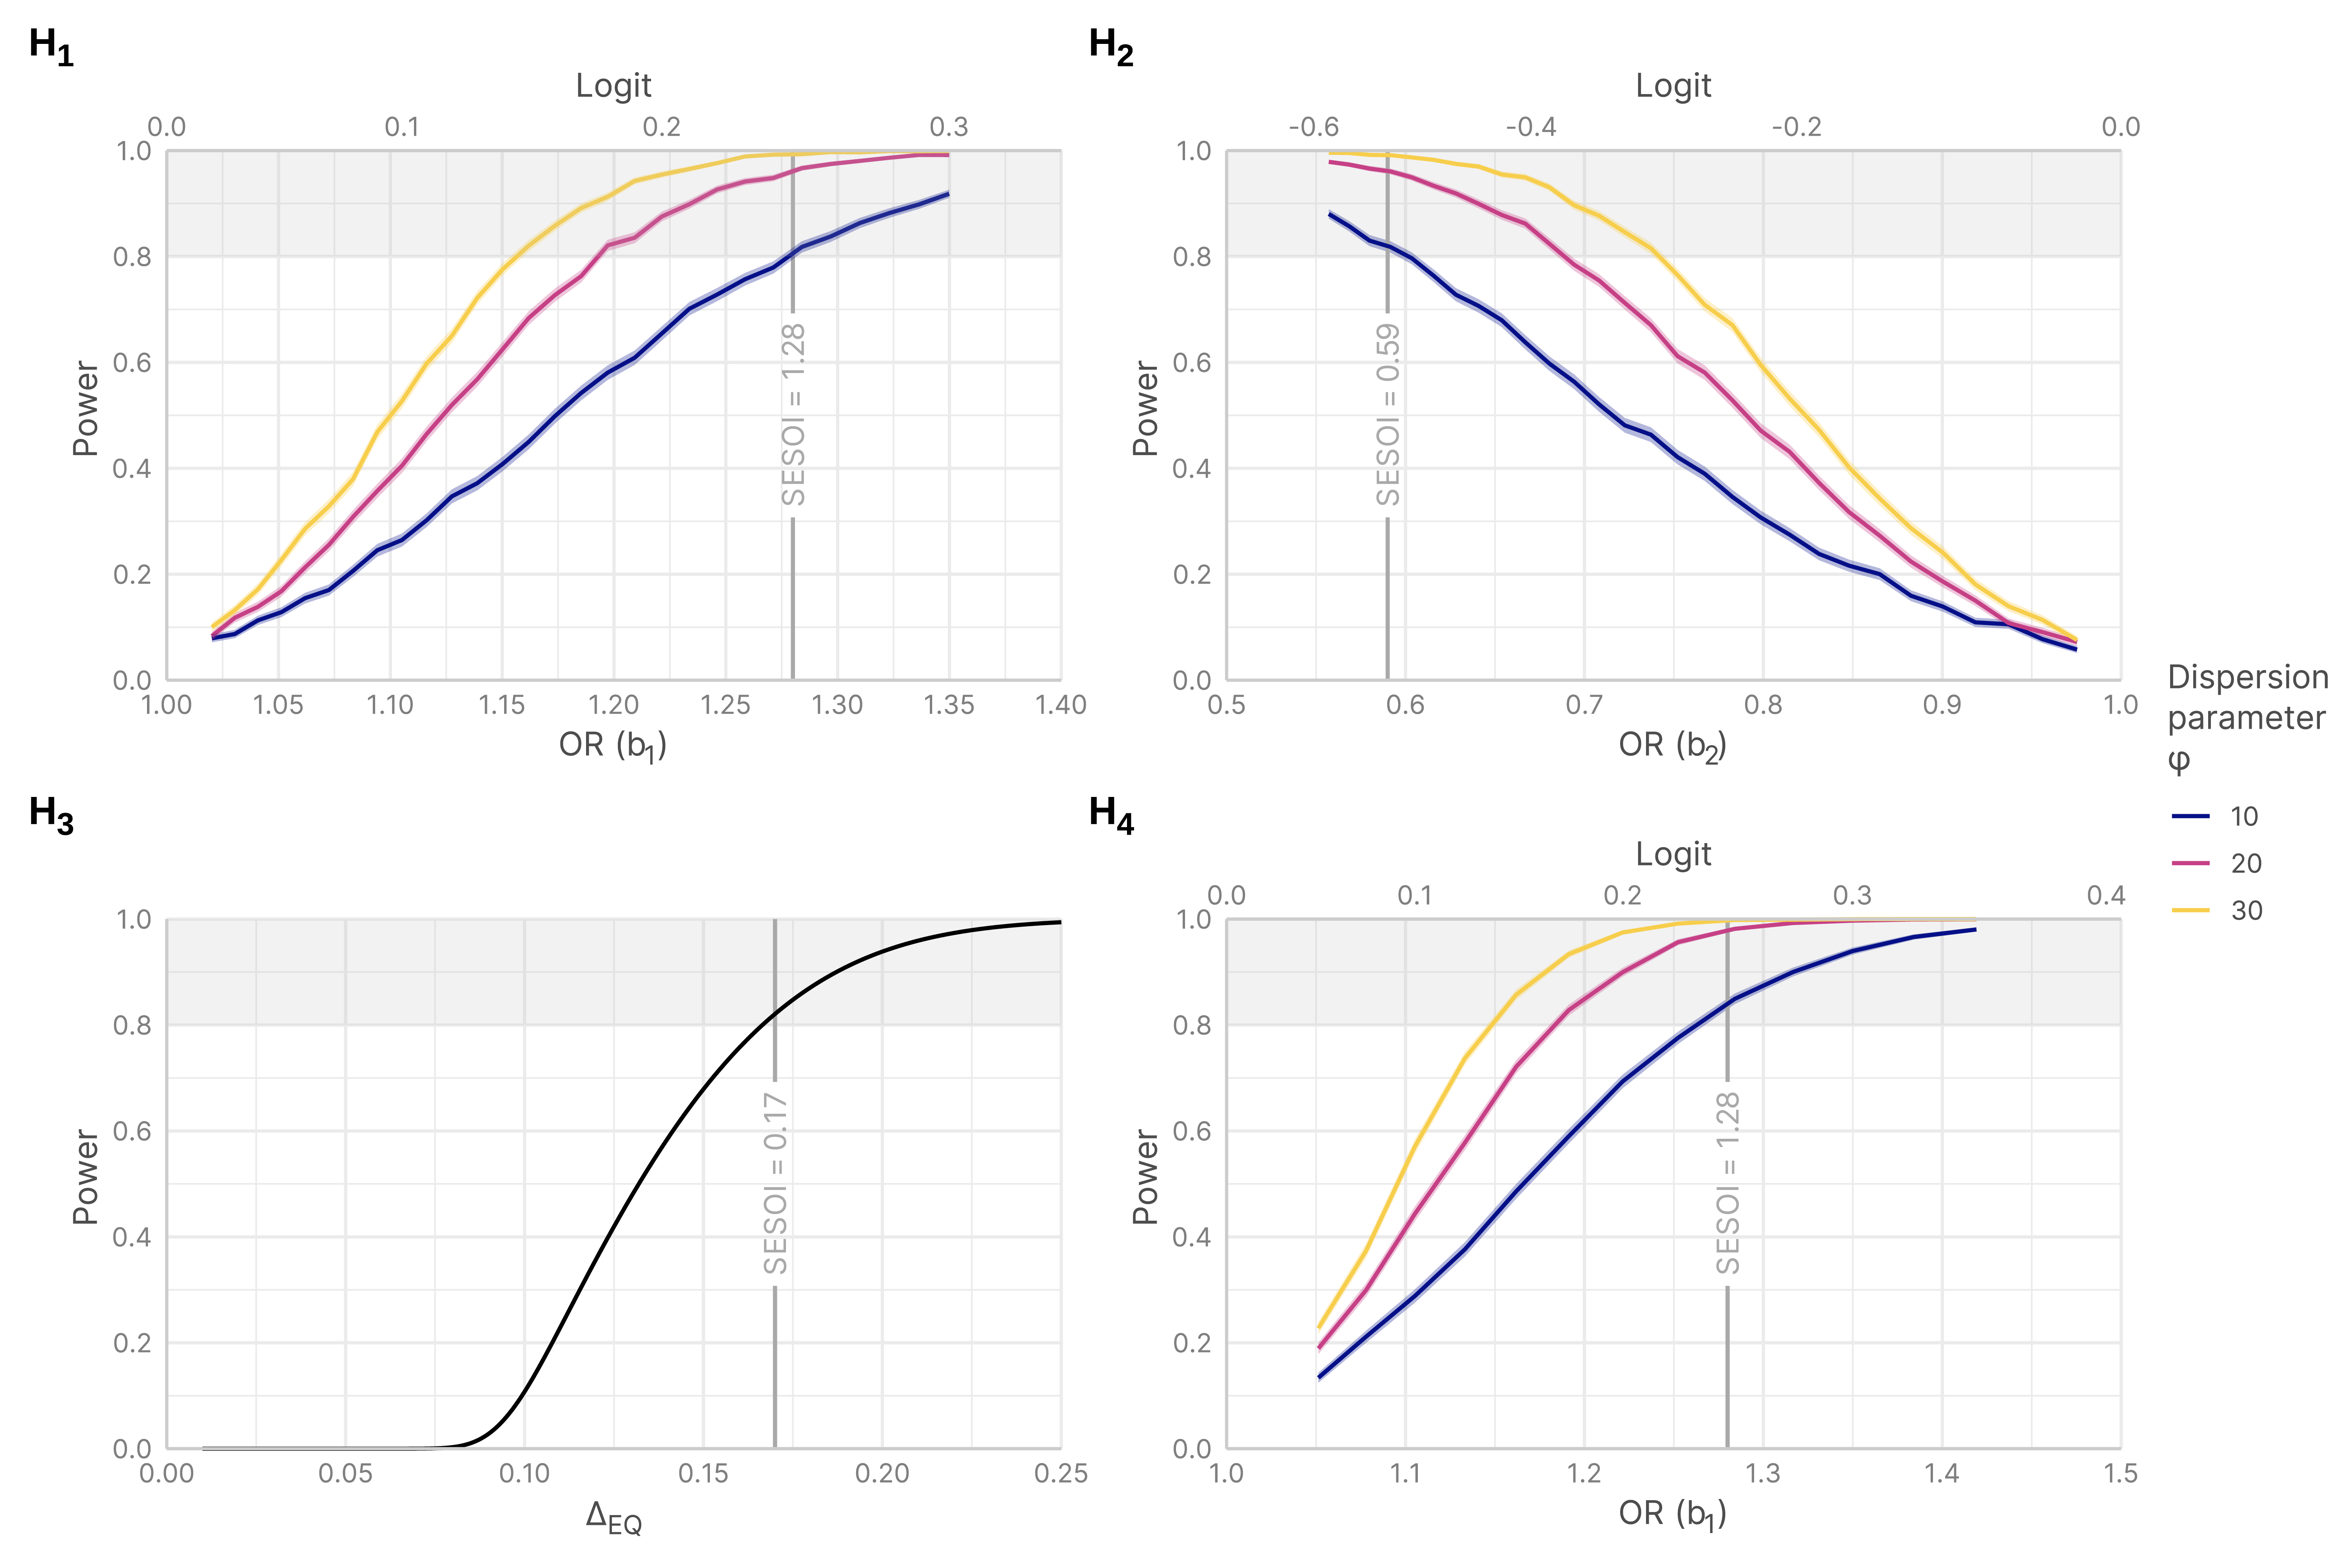
\includegraphics[width=1\textwidth,height=\textheight]{../figures/power_sesoi.png}
\end{center}

\begingroup
\scriptsize
\textit{Note.} OR: Odds ratio. Ribbons around the lines represent the 95\\% confidence interval. 
\endgroup
\end{figure}

\subsection{Appendix B: Research Transparency
Statement}\label{appendix-b-research-transparency-statement}

The present thesis project was aimed to to be as transparent and
reproducible as possible. The preregistration of the study, all data,
code, and supplementary files needed to reproduce the results of this
study are openly available on the zugehörigen
\href{https://osf.io/87m9k/?view_only=030c8d1c46474270b5886c4dfc491a78}{OSF
repository} of this thesis
(https://osf.io/87m9k/?view\_only=030c8d1c46474270b5886c4dfc491a78) and
on \href{https://github.com/jlschnatz/bachelor-thesis}{GitHub}.To
enhance the reproducability of this project, all analyses, figures, the
thesis manuscript itself are generated within a containerized software
environment using \emph{Docker}
(\citeproc{ref-merkel_docker_2014}{Merkel, 2014}). The workflow for the
analyses was explicitely management using \emph{Snakemake}
(\citeproc{ref-molder_sustainable_2021}{Mölder et al., 2021}) and the R
packages dependencies and version management used for the statistical
analyses were managemed using \emph{renv}
(\citeproc{ref-ushey_renv_2024}{Ushey \& Wickham, 2024}). The thesis
manuscript itself is dynamically generated and reproducible using the
\emph{Quarto} publishing system.

\begin{itemize}
\tightlist
\item
  The project is fully st containerized using \emph{Docker}
  (\citeproc{ref-merkel_docker_2014}{Merkel, 2014})
\item
  Software and operating system virtualization, fully containerized
  project using Docker R package dependencies and version management
  using \emph{renv} (\citeproc{ref-ushey_renv_2024}{Ushey \& Wickham,
  2024}).
\item
  Data analysis workflow management tool \emph{Snakemake}
  (\citeproc{ref-molder_sustainable_2021}{Mölder et al., 2021})
\item
  thesis is written using the \emph{Quarto}
  (\citeproc{ref-allaire_quarto_2024}{Allaire et al., 2024}) open-source
  scientific and technical publishing system
\end{itemize}

CITE: All analyses, figures, and the final manuscript were generated
using a makefile, bash scripts, and R and Rmarkdown. All relevant
metadata, as well as analysis and manuscript code, are available on
GitHub: https://github.com/ZimmermanLab/SF-metrosideros-endophytes/ and
archived at Zenodo (https://doi.org/10.5281/zenodo.8075450). The
complete computational environment for the analyses is documented in a
Dockerfile based on rocker containers (Boettiger, 2014) and a renv.lock
(Ushey, 2021) file in that same repository.

\subsection{Appendix C: Deviations of
Preregistration}\label{appendix-c-deviations-of-preregistration}

\subsection{Appendix D: Test}\label{appendix-d-test}

\begin{table}[H]
\centering
\caption{\label{tab:unnamed-chunk-42}Estimated Parameters for the Distribution of Effect Size and Sample Size from each Meta-Analysis via ML}
\centering
\resizebox{\ifdim\width>\linewidth\linewidth\else\width\fi}{!}{
\begin{threeparttable}
\begin{tabular}[t]{>{\raggedright\arraybackslash}p{5.33cm}>{\centering\arraybackslash}p{5.33cm}>{\centering\arraybackslash}p{5.33cm}}
\toprule
Parameter & Minimum & Maximum\\
\midrule
\addlinespace[0.3em]
\multicolumn{3}{l}{\textbf{Effect Size}}\\
\hspace{1em}$\widehat{\mu}_d$ & -1.911 & 2.599\\
\hspace{1em}$\widehat{\sigma}^2_d$ & 0.003 & 4.349\\
\addlinespace[0.3em]
\multicolumn{3}{l}{\textbf{Sample Size}}\\
\hspace{1em}$\widehat{\phi}_n$ & 0.042 & 176.620\\
\hspace{1em}$\widehat{\mu}_n$ & 17.365 & 1438.443\\
\bottomrule
\end{tabular}
\begin{tablenotes}
\item \textit{Note.} Maximum Likelihood Estimation using the Nelder-Mead optimizer.
\end{tablenotes}
\end{threeparttable}}
\end{table}

\subsection{Appendix E: Regression Tables of Confirmatory
Analyses}\label{appendix-e-regression-tables-of-confirmatory-analyses}

\begin{table}[H]
\centering
\caption{Beta Regression Results for $\mathcal{H}_1$}
\centering
\resizebox{\ifdim\width>\linewidth\linewidth\else\width\fi}{!}{
\begin{threeparttable}
\begin{tabular}[t]{>{\raggedright\arraybackslash}p{2.66cm}>{\centering\arraybackslash}p{2.66cm}>{\centering\arraybackslash}p{2.66cm}>{\centering\arraybackslash}p{2.66cm}>{\centering\arraybackslash}p{2.66cm}>{\centering\arraybackslash}p{2.66cm}}
\toprule
Term & Estimate & $CI$ (95\%) & $SE$ & $z$ & $p$\\
\midrule
\addlinespace[0.3em]
\multicolumn{6}{l}{\textbf{Mean model component: $\mu$}}\\
\\[-1.5ex]\hspace{1em}Intercept & $4.05^a$ & {}[3.16, 5.19] & 0.13 & 11.07 & < .001\\
\hspace{1em}$z_{r_s}$ & $2.22^a$ & $[1.38, Inf]^c$ & 0.29 & 2.74 & .035\\
\addlinespace[0.3em]
\multicolumn{6}{l}{\textbf{Precision model component: $\phi$}}\\
\\[-1.5ex]\hspace{1em}Intercept & $5.84^b$ & {}[3.95, 8.63] & 0.20 & 8.85 & < .001\\
\bottomrule
\end{tabular}
\begin{tablenotes}[flushleft]
\item \textit{Note.} $LL$ = 132.03, $MAE$ = 0.21, $AIC$ = -258.06, $BIC$ = -249.03, $R^2$ = 0.051
\item[a] $OR$
\item[b] Identity
\item[c] One-sided Confidence interval in direction of the hypothesis
\end{tablenotes}
\end{threeparttable}}
\end{table}

\begin{table}[H]
\centering
\caption{Beta Regression Results for $\mathcal{H}_2$}
\centering
\resizebox{\ifdim\width>\linewidth\linewidth\else\width\fi}{!}{
\begin{threeparttable}
\begin{tabular}[t]{>{\raggedright\arraybackslash}p{2.66cm}>{\centering\arraybackslash}p{2.66cm}>{\centering\arraybackslash}p{2.66cm}>{\centering\arraybackslash}p{2.66cm}>{\centering\arraybackslash}p{2.66cm}>{\centering\arraybackslash}p{2.66cm}}
\toprule
Term & Estimate & $CI$ (95\%) & $SE$ & $z$ & $p$\\
\midrule
\addlinespace[0.3em]
\multicolumn{6}{l}{\textbf{Mean model component: $\mu$}}\\
\\[-1.5ex]\hspace{1em}Intercept & $3.30^a$ & {}[2.71, 4.03] & 0.10 & 11.79 & < .001\\
\hspace{1em}$\Delta_{\mu_d}^2$ & $0.04^a$ & $[0.00, 0.73]^c$ & 1.84 & -1.81 & .035\\
\addlinespace[0.3em]
\multicolumn{6}{l}{\textbf{Precision model component: $\phi$}}\\
\\[-1.5ex]\hspace{1em}Intercept & $4.85^b$ & {}[3.63, 6.47] & 0.15 & 10.70 & < .001\\
\bottomrule
\end{tabular}
\begin{tablenotes}[flushleft]
\item \textit{Note.} $LL$ = 164.25, $MAE$ = 0.23, $AIC$ = -322.51, $BIC$ = -312.51, $R^2$ = 0.026
\item[a] $OR$
\item[b] Identity
\item[c] One-sided Confidence interval in direction of the hypothesis
\end{tablenotes}
\end{threeparttable}}
\end{table}

\begin{table}[H]
\centering
\caption{Two One-Sided Tests Result for $\mathcal{H}_3$}
\centering
\resizebox{\ifdim\width>\linewidth\linewidth\else\width\fi}{!}{
\begin{threeparttable}
\begin{tabular}[t]{>{\raggedright\arraybackslash}p{3.2cm}>{\centering\arraybackslash}p{3.2cm}>{\centering\arraybackslash}p{3.2cm}>{\centering\arraybackslash}p{3.2cm}>{\centering\arraybackslash}p{3.2cm}}
\toprule
Type & $t$ & $SE$ & $df$ & $p$\\
\midrule
NHST & -2.36 & 0.009 & 56 & .022\\
TOST $\Delta < \Delta_L$ & 17.30 & 0.009 & 56 & < .001\\
TOST $\Delta > \Delta_L$ & -22.02 & 0.009 & 56 & < .001\\
\bottomrule
\end{tabular}
\begin{tablenotes}[flushleft]
\item \textit{Note.} NHST: Null Hypothesis Significance Test, TOST: Two One-Sided Test
\end{tablenotes}
\end{threeparttable}}
\end{table}

\begin{table}[H]
\centering
\caption{Beta Regression Results for $\mathcal{H}_4$}
\centering
\resizebox{\ifdim\width>\linewidth\linewidth\else\width\fi}{!}{
\begin{threeparttable}
\begin{tabular}[t]{>{\raggedright\arraybackslash}p{2.66cm}>{\centering\arraybackslash}p{2.66cm}>{\centering\arraybackslash}p{2.66cm}>{\centering\arraybackslash}p{2.66cm}>{\centering\arraybackslash}p{2.66cm}>{\centering\arraybackslash}p{2.66cm}}
\toprule
Term & Estimate & $CI$ (95\%) & $SE$ & $z$ & $p$\\
\midrule
\addlinespace[0.3em]
\multicolumn{6}{l}{\textbf{Mean model component: $\mu$}}\\
\\[-1.5ex]\hspace{1em}Intercept & $3.30^a$ & {}[2.67, 4.08] & 0.11 & 11.07 & < .001\\
\addlinespace[0.3em]
\multicolumn{6}{l}{Research Synthesis Type}\\
\\[-1.5ex]\hspace{1em}\hspace{1em}Meta-Analyses &  &  &  &  & \\
\hspace{1em}\hspace{1em}RRR & $0.81^a$ & $[0.61, Inf]^c$ & 0.18 & -1.17 & .879\\
\addlinespace[0.3em]
\multicolumn{6}{l}{\textbf{Precision model component: $\phi$}}\\
\\[-1.5ex]\hspace{1em}Intercept & $4.79^b$ & {}[3.59, 6.38] & 0.15 & 10.71 & < .001\\
\bottomrule
\end{tabular}
\begin{tablenotes}[flushleft]
\item \textit{Note.} MR: Multisite Replication; $LL$ = 163.31, $MAE$ = 0.23, $AIC$ = -320.62, $BIC$ = -310.62, $R^2$ = 0.011
\item[a] $OR$
\item[b] Identity
\item[c] One-sided Confidence interval in direction of the hypothesis
\end{tablenotes}
\end{threeparttable}}
\end{table}

\section*{Eidesstattliche Erklärung}\label{eidesstattliche-erkluxe4rung}

Ich versichere hiermit, dass ich die vorliegende Arbeit selbständig und
ohne Benutzung anderer als der angegebenen Quellen und Hilfsmittel
verfasst habe. Wörtlich übernommene Sätze oder Satzteile sind als Zitat
belegt, andere Anlehnungen, hinsichtlich Aussage und Umfang, unter
Quellenangabe kenntlich gemacht. Die Aufgabenstellung habe ich alleine
und ohne Besprechung mit anderen bearbeitet.

Die Arbeit hat in gleicher oder ähnlicher Form noch keiner
Prüfungsbehörde vorgelegen und ist nicht veröffentlicht. Sie wurde
nicht, auch nicht auszugsweise, für eine andere Prüfungs- oder
Studienleistung verwendet.

\bigskip
\bigskip

\noindent{Datum: 18. Mai, 2024}

\bigskip

\noindent{Unterschrift:}



\end{document}
